\documentclass[a4paper,11pt,bibliography=totoc,listof=totoc,headinclude=true,cleardoublepage=empty,oneside]{scrbook}
% Option "oneside" für einseitigen Druck. Weglassen, falls die Arbeit doppelseitig gedruckt wird

\usepackage[english,ngerman]{babel}
\usepackage[utf8]{inputenc}
\usepackage{ifthen}
\usepackage{xcolor}
\usepackage{amsmath,amsthm,amssymb,amsfonts}
\usepackage{graphicx}
\graphicspath{{../abbildungen/}{./}}
\usepackage{psfrag}
\usepackage{tikz, pgfplots}

\usepackage[T1]{fontenc}
\renewcommand{\familydefault}{cmss} % Schriftart


\usepackage{mathtools}     
\usepackage{booktabs}       
\usepackage{subcaption}     

%%%%%%%%%%%%%%%%%%%%%%%%%%%%%%%%%%%%%%%%%%%%%%%%%%%%%%%%%%%%%%%%%%%%%%%%%%%%%%%
% ARBEITSHILFE: QUELLENBLOCK
%
% \quellen{...} setzt einen kleinen blauen Kasten mit den Belegstellen unter
% eine Abschnittsueberschrift. Beim Schreiben hat man die Referenzen direkt vor
% Augen. VOR DER ABGABE: die \renewcommand-Zeile aktivieren -- dann
% verschwinden alle Bloecke aus dem PDF, ohne dass man sie einzeln loeschen muss.
%%%%%%%%%%%%%%%%%%%%%%%%%%%%%%%%%%%%%%%%%%%%%%%%%%%%%%%%%%%%%%%%%%%%%%%%%%%%%%%

\newcommand{\quellen}[1]{%
  \par\smallskip
  {\color{uhh_blue}\small\textbf{Belegstellen.}\ #1}%
  \par\medskip}
% \renewcommand{\quellen}[1]{} % <-- vor der Abgabe aktivieren

%%%%%%%%%%%%%%%%%%%%%%%%%%%%%%%%%%%%%%%%%%%%%%%%%%%%%%%%%%%%%%%%%%%%%%%%%%%%%%%
% ARBEITSHILFE: ANMERKUNGEN
%
% \anmerkung{...} setzt eine Arbeitsnotiz als orangen Fliesstext.
% VOR DER ABGABE: die \renewcommand-Zeile aktivieren, dann verschwinden alle
% Anmerkungen aus dem PDF, ohne dass man sie einzeln loeschen muss.
%%%%%%%%%%%%%%%%%%%%%%%%%%%%%%%%%%%%%%%%%%%%%%%%%%%%%%%%%%%%%%%%%%%%%%%%%%%%%%%

\newcommand{\anmerkung}[1]{%
  \par\smallskip
  {\color{uhh_red}\small\textbf{Anmerkung.}\ #1}%
  \par\medskip}
% \renewcommand{\anmerkung}[1]{} % <-- vor der Abgabe aktivieren


\theoremstyle{plain}
\newtheorem{Satz}{Satz}[chapter]
\newtheorem{Lemma}[Satz]{Lemma}
\newtheorem{Proposition}[Satz]{Proposition}
\newtheorem{Korollar}[Satz]{Korollar}

\theoremstyle{definition}
\newtheorem{Definition}[Satz]{Definition}
\newtheorem{Beispiel}[Satz]{Beispiel}
\newtheorem{Bemerkung}[Satz]{Bemerkung}
\newtheorem{Algorithmus}[Satz]{Algorithmus}

\renewcommand{\proofname}{Beweis}

%%%%%%%%%%%%%%%%%%%%%%%%%%%%%%%%%%%%%%%%%%%%%%%%%%%%%%%%%%%%%%%%%%%%%%%%%%%%%%%
% EIGENE ABKUERZUNGEN
%%%%%%%%%%%%%%%%%%%%%%%%%%%%%%%%%%%%%%%%%%%%%%%%%%%%%%%%%%%%%%%%%%%%%%%%%%%%%%%

\newcommand{\R}{\mathbb{R}}
\newcommand{\Z}{\mathbb{Z}}
\newcommand{\N}{\mathbb{N}}
\newcommand{\C}{\mathbb{C}}
\newcommand{\LZwei}{L^2(\R)}
\newcommand{\ellZwei}{\ell^2(\Z)}
\newcommand{\scal}[2]{\langle #1, #2 \rangle}
\newcommand{\norm}[1]{\lVert #1 \rVert}
\newcommand{\abs}[1]{\lvert #1 \rvert}
\DeclareMathOperator{\supp}{supp}
\DeclareMathOperator{\MAD}{MAD}
\DeclareMathOperator{\SNR}{SNR}
\DeclareMathOperator{\MSE}{MSE}
\DeclareMathOperator{\sgn}{sgn}


\definecolor{uhh_red}{RGB}{226,0,26}
\definecolor{uhh_blue}{RGB}{2,113,187}
\definecolor{uhh_grey}{RGB}{59,81,91}

\definecolor{change}{RGB}{2,113,187}

\def\revision#1{{\color{uhh_red}#1}}

\usepackage{hyperref}

\hypersetup{
    colorlinks=true,
    linkcolor=orange,
    citecolor=orange,
    filecolor=orange,
    urlcolor=purple,
    unicode,
    }

% Zum Druck verwende schwarze Links!
%\usepackage[unicode,colorlinks=true,linkcolor=black,citecolor=black,urlcolor=black,pagebackref=false]{hyperref}

% document style
\KOMAoptions{footinclude=false} % Fusszeile wird nicht zu Satzspiegel gezaehlt
\KOMAoptions{headsepline=true} % Trennlinie zwischen Kopfzeile und Text
\KOMAoptions{DIV=12} % beeinflusst Satzspiegel
\KOMAoptions{BCOR=8mm} % Bindekorrektur
\pagestyle{headings} % mit Kopfzeilen

\recalctypearea % berechne Satzspiegel neu

%haar beispiel 
\newcommand{\haarplot}[3]{% #1 = a > 0, #2 = b, #3 = Beschriftung
  \pgfmathsetmacro{\haaramp}{1/sqrt(abs(#1))}
  \pgfmathsetmacro{\haarxO}{#2}
  \pgfmathsetmacro{\haarxM}{#2+0.5*(#1)}
  \pgfmathsetmacro{\haarxE}{#2+(#1)}
  \draw[gray!45, dashed, line width=0.4pt] (-1,1) -- (3.6,1);
  \draw[gray!45, dashed, line width=0.4pt] (-1,-1) -- (3.6,-1);
  \draw[-latex, line width=0.5pt] (-1,0) -- (3.8,0)
        node[below right, font=\footnotesize] {$t$};
  \draw[-latex, line width=0.5pt] (0,-1.9) -- (0,1.9);
  \foreach \x in {1,2,3} \draw (\x,0.07) -- (\x,-0.07)
        node[below, font=\scriptsize] {$\x$};
  \draw[uhh_blue, line width=1.1pt] (-1,0) -- (\haarxO,0);
  \draw[uhh_blue, line width=1.1pt] (\haarxE,0) -- (3.8,0);
  \draw[uhh_blue, line width=1.1pt] (\haarxO,\haaramp) -- (\haarxM,\haaramp);
  \draw[uhh_blue, line width=1.1pt] (\haarxM,-\haaramp) -- (\haarxE,-\haaramp);
  \draw[uhh_blue, dotted] (\haarxO,0) -- (\haarxO,\haaramp);
  \draw[uhh_blue, dotted] (\haarxM,\haaramp) -- (\haarxM,-\haaramp);
  \draw[uhh_blue, dotted] (\haarxE,-\haaramp) -- (\haarxE,0);
  \fill[uhh_blue] (\haarxO,\haaramp) circle (1.3pt);
  \draw[uhh_blue, fill=white] (\haarxM,\haaramp) circle (1.3pt);
  \fill[uhh_blue] (\haarxM,-\haaramp) circle (1.3pt);
  \draw[uhh_blue, fill=white] (\haarxE,-\haaramp) circle (1.3pt);
  \node[font=\small, anchor=north] at (1.4,-2.15) {#3};
}

%%%%%%%%%%%%%%%%%%%%%%%%%%%%%%%%%%%%%%%%%%%%%%%%%%%%%%%%%%%%%%%%%%%%%%%%%%%%%%%
%%%%%%%%%%%%%%%%%%%%%%%%%%%%%%%%%%%%%%%%%%%%%%%%%%%%%%%%%%%%%%%%%%%%%%%%%%%%%%%

\begin{document}

%%%%%%%%%%%%%%%%%%%%%%%%%%%%%%%%%%%%%%%%%%%%%%%%%%%%%%%%%%%%%%%%%%%%%%%%%%%%%%%
% TITELSEITE [OBLIGATORISCH]
%%%%%%%%%%%%%%%%%%%%%%%%%%%%%%%%%%%%%%%%%%%%%%%%%%%%%%%%%%%%%%%%%%%%%%%%%%%%%%%

\pagenumbering{Alph}
\selectlanguage{ngerman}

\begin{titlepage}
  \begin{center}
    
\includegraphics[width=0.45\textwidth]{uhh-logo.png}
    \vskip 1cm%
    {\LARGE B~\Large A~C~H~E~L~O~R~A~R~B~E~I~T}
    \vskip 8mm
    {\huge\bfseries\color{change}Entrauschung von EKG-Signalen \\[1ex] mittels 
    der diskreten Wavelet-Transformation}
    \vskip 1cm
    \large
    ausgef\"uhrt am
    \vskip 0.75cm
    {\Large Fachbereich Mathematik}\\[1ex]
    {\Large Fakultät für Mathematik, Informatik und Naturwissenschaften}\\[1ex]
    {\Large Universität Hamburg}
    \vskip0.75cm
    unter der Anleitung von
    \vskip0.75cm
    {\Large\bfseries\color{change}Name des Betreuers}\\[1ex]
    \vskip 0.5cm
    durch
    \vskip 0.5cm
    {\Large\bfseries\color{change}Hilda Beuting}\\[1ex]
    Matrikelnummer: {\color{change}12345678}\\[1ex]
    {\color{change}Straße und Hausnummer}\\[1ex]
    {\color{change}PLZ und Ort}
  \end{center}

  \vfill

  \small
  Hamburg, am {\color{change} Datum} %\today
  \vspace*{-15mm}
\end{titlepage}

\cleardoublepage

%%%%%%%%%%%%%%%%%%%%%%%%%%%%%%%%%%%%%%%%%%%%%%%%%%%%%%%%%%%%%%%%%%%%%%%%%%%%%%%
% INHALTSVERZEICHNIS [OBLIGATORISCH]
%%%%%%%%%%%%%%%%%%%%%%%%%%%%%%%%%%%%%%%%%%%%%%%%%%%%%%%%%%%%%%%%%%%%%%%%%%%%%%%

\pagenumbering{roman}
\selectlanguage{ngerman}

\tableofcontents

\cleardoublepage
\pagenumbering{arabic}

%%%%%%%%%%%%%%%%%%%%%%%%%%%%%%%%%%%%%%%%%%%%%%%%%%%%%%%%%%%%%%%%%%%%%%%%%%%%%%%
%%%%%%%%%%%%%%%%%%%%%%%%%%%%%%%%%%%%%%%%%%%%%%%%%%%%%%%%%%%%%%%%%%%%%%%%%%%%%%%
\chapter{Einleitung}
\label{chapter:einleitung}
%%%%%%%%%%%%%%%%%%%%%%%%%%%%%%%%%%%%%%%%%%%%%%%%%%%%%%%%%%%%%%%%%%%%%%%%%%%%%%%
%%%%%%%%%%%%%%%%%%%%%%%%%%%%%%%%%%%%%%%%%%%%%%%%%%%%%%%%%%%%%%%%%%%%%%%%%%%%%%%

\anmerkung{Einleitung ganz zum Schluss schreiben. Laut Vorlage muss hier
stehen: (a) Worum geht es, (b) Einordnung ins Forschungsfeld, (c) Fragestellung,
(d) Relevanz, (e) vorhandene Literatur, (f) EIGENER ANTEIL der Arbeit,
(g) grober Aufbau der Arbeit.}

%%%%%%%%%%%%%%%%%%%%%%%%%%%%%%%%%%%%%%%%%%%%%%%%%%%%%%%%%%%%%%%%%%%%%%%%%%%%%%%
\section{Motivation: EKG-Signale und ihre Störquellen}
%%%%%%%%%%%%%%%%%%%%%%%%%%%%%%%%%%%%%%%%%%%%%%%%%%%%%%%%%%%%%%%%%%%%%%%%%%%%%%%

\anmerkung{EKG-Signale und ihre Störquellen Das EKG ist ein nichtstationäres 
biomedizinisches Signal, dessen diagnostisch entscheidende Strukturen von 
Störungen überlagert werden, die im selben Frequenzband liegen wie das 
Nutzsignal — womit einfache Frequenzfilter ausscheiden.}

\anmerkung{hier schon kurzer aufbau ekg signal kurzer qrskomplex und langer t p welle... }

\quellen{ \begin{itemize}
  \item LMR, Kap. 3.1.2 „EKG-Analyse", S. 238–240 [bestätigt] — Herzklappenrhythmus 
        und „late potentials" als diagnostische Fragestellungen; Abb. 3.1 (S. 239)  
  \item Gacek, Kap. 2.1, S. 21–22 [bestätigt] — diagnostische Bedeutung, historische 
        Einordnung
  \item Gacek, Kap. 2.3, S. 25–27 [bestätigt] — Störquellen im Überblick
  \item Chatterjee, Kap. 1.1 „Predominant noises in ECG", S. 570 [bestätigt]
  \item Aqil, Kap. 2, S. 53–54 [bestätigt] — Fig. 3, Rauschtypen
  \item Rebstadt, Kap. 2.1, S. 7–11 [bestätigt] — Abb. 2.3 (S. 10)
          \end{itemize}
        }

%%%%%%%%%%%%%%%%%%%%%%%%%%%%%%%%%%%%%%%%%%%%%%%%%%%%%%%%%%%%%%%%%%%%%%%%%%%%%%%
\section{Warum die Fourier-Analyse nicht genügt}
\label{sec:fourier-grenzen}
%%%%%%%%%%%%%%%%%%%%%%%%%%%%%%%%%%%%%%%%%%%%%%%%%%%%%%%%%%%%%%%%%%%%%%%%%%%%%%%
\anmerkung{VERSCHOBEN aus dem alten Abschnitt~2.5. Begründung: In Kapitel~2 war das
ein Fremdkörper -- dort werden Werkzeuge bereitgestellt, hier wird die Fragestellung
motiviert. Der Abschnitt liefert genau das Argument, das die ganze Arbeit trägt:
Die Fourier-Basis sagt, \emph{welche} Frequenzen auftreten, nicht \emph{wann}.}
\anmerkung{Die Fourier-Basis ist global; sie sagt welche Frequenzen auftreten, nicht wann 
— bei einem QRS-Komplex ist genau die Lokalisierung entscheidend.}
\quellen{
  \begin{itemize}
    \item LMR, Kap. 1.3.2 „Wavelet-Transformation und gefensterte Fourier-Transformation", 
    S. 36–37 [bestätigt] — direkter Vergleich beider Transformationen, in der 2. Auflage 
    eigens dafür neu aufgenommen
    \item LMR, Kap. 1.3.1 „Phasenraumdarstellung", S. 30–35 [bestätigt]
    \item LMR, Vorwort zur ersten Auflage, S. 3 [bestätigt] — fehlende 
    Lokalisierungseigenschaft der Fourier-Transformation, prägnant formuliert
    \item Blatter, Kap. 1.4, S. 10–12 [bestätigt]; Kap. 2.3 „Heisenbergsche Unschärferelation", 
    S. 43–46 [bestätigt]
    \item SteinShakarchi, Kap. 5.4, S. 158–160 [bestätigt]
    \item HankeBourgeois, Beispiel 52.7 mit Abbildung 52.1, S. 403–404 [bestätigt] — reales 
    EKG-Signal mit $N = 2048$
          Meßwerten und seinen Bestapproximationen aus $T_8$ und $T_{32}$
          ; die scharfen Peaks werden mit sinkendem Polynomgrad ausgeglättet, 
          $t_8$ „übersieht" das Minimum am ca. 200. Datenpunkt
    \item HankeBourgeois, S. 433–434 [bestätigt] — quantitativ: die Fourierkoeffizienten 
    von $\chi_{[a,b]}$ fallen nur wie $1/k$, der $L^2$-Fehler nach $n$ Termen ist 
    $\sim n^{-1/2}$; „schlechte Lokalisierungseigenschaft bezüglich der Ortsvariablen"
    \item HankeBourgeois, Beispiel 56.3 mit Abbildung 56.2, S. 440 [bestätigt] — Fourier- 
    vs. Waveletkoeffizienten desselben EKG-Signals in logarithmischer Skala
    \item Rebstadt, Abb. 2.7, S. 22 [bestätigt]
    \item Fußnote S. 404: Die EKG-Daten stammen laut HankeBourgeois von Prof. Dr. P. Maaß, 
    Universität Bremen — demselben Maaß wie in Louis/Maaß/Rieder. Deine beiden 
    deutschsprachigen Quellen arbeiten am selben Signal.
  \end{itemize}
}
%%%%%%%%%%%%%%%%%%%%%%%%%%%%%%%%%%%%%%%%%%%%%%%%%%%%%%%%%%%%%%%%%%%%%%%%%%%%%%%
\section{Zielsetzung und Abgrenzung}
%%%%%%%%%%%%%%%%%%%%%%%%%%%%%%%%%%%%%%%%%%%%%%%%%%%%%%%%%%%%%%%%%%%%%%%%%%%%%%%

\anmerkung{Ziel ist die mathematisch vollständige Herleitung der DWT-Entrauschung; 
Abgrenzung gegenüber konkurrierenden Verfahren, die nur benannt werden.}

\quellen{ \begin{itemize}
  \item LMR, Vorwort zur ersten Auflage, S. 3–4 [bestätigt] — Verzahnung von 
  Theorie und Anwendung als Programm
  \item Chatterjee, Kap. 2–4, S. 571–581
  \item Rebstadt, Kap. 2.3, S. 14–31 [bestätigt]
         \end{itemize}
        }

%%%%%%%%%%%%%%%%%%%%%%%%%%%%%%%%%%%%%%%%%%%%%%%%%%%%%%%%%%%%%%%%%%%%%%%%%%%%%%%
\section{Aufbau der Arbeit}
%%%%%%%%%%%%%%%%%%%%%%%%%%%%%%%%%%%%%%%%%%%%%%%%%%%%%%%%%%%%%%%%%%%%%%%%%%%%%%%

%%%%%%%%%%%%%%%%%%%%%%%%%%%%%%%%%%%%%%%%%%%%%%%%%%%%%%%%%%%%%%%%%%%%%%%%%%%%%%%
%%%%%%%%%%%%%%%%%%%%%%%%%%%%%%%%%%%%%%%%%%%%%%%%%%%%%%%%%%%%%%%%%%%%%%%%%%%%%%%
\chapter{Funktionalanalytische Grundlagen}
\label{chapter:grundlagen}
%%%%%%%%%%%%%%%%%%%%%%%%%%%%%%%%%%%%%%%%%%%%%%%%%%%%%%%%%%%%%%%%%%%%%%%%%%%%%%%
%%%%%%%%%%%%%%%%%%%%%%%%%%%%%%%%%%%%%%%%%%%%%%%%%%%%%%%%%%%%%%%%%%%%%%%%%%%%%%%

\anmerkung{Block A. Kapiteleinleitung: Ziel ist der funktionalanalytische
Rahmen, in dem die Wavelet-Transformation als unitäre Abbildung erscheint.}

%%%%%%%%%%%%%%%%%%%%%%%%%%%%%%%%%%%%%%%%%%%%%%%%%%%%%%%%%%%%%%%%%%%%%%%%%%%%%%%
\section{Der Hilbertraum \texorpdfstring{$L^2(\R)$}{L2(R)}}
%%%%%%%%%%%%%%%%%%%%%%%%%%%%%%%%%%%%%%%%%%%%%%%%%%%%%%%%%%%%%%%%%%%%%%%%%%%%%%%
\anmerkung{Einführung von $L^2(\R)$ als vollständigem Raum mit Skalarprodukt — 
dem Raum, in dem sämtliche Signale und Wavelets im Folgenden leben.}

\quellen{
  \begin{itemize}
    \item Serov, Kap. 25, S. 249–253 [bestätigt] (Def. 25.1 Skalarprodukt, Def. 
          25.7 Hilbertraum)
    \item Blatter, Kap. 2.1, S. 26–27 [bestätigt]
    \item LMR, „Notationen", S. 9–12 [bestätigt] — Räume $L^p, C^(\infty), S(\R), 
          S'(\R)$ in genau der Notation, die LMR durchgehend verwendet
  \end{itemize}
}
%%%%%%%%%%%%%%%%%%%%%%%%%%%%%%%%%%%%%%%%%%%%%%%%%%%%%%%%%%%%%%%%%%%%%%%%%%%%%%%
\section{Orthonormalbasen und ihre Charakterisierung}
%%%%%%%%%%%%%%%%%%%%%%%%%%%%%%%%%%%%%%%%%%%%%%%%%%%%%%%%%%%%%%%%%%%%%%%%%%%%%%%
\anmerkung{Der zentrale Satz: Vollständigkeit, Parseval-Gleichung und die 
Entwicklung jedes Elements sind für ein Orthonormalsystem äquivalent.}
\quellen{
  \begin{itemize}
    \item Serov, Satz 25.18 „Characterization of an orthonormal basis", S. 258 [bestätigt]
    \item Serov, Def. 25.16–25.17, S. 257–258 [bestätigt]
    \item Serov, Satz 25.12 (Projektionssatz), S. 254–255 [geschätzt]
    \item Blatter, Kap. 2.1, S. 27 [bestätigt]
    \item HankeBourgeois, Satz 31.6, S. 281 [bestätigt] — (a) Entwicklung, 
    (b) Satz des Pythagoras, (c) Bestapproximation, (d) Besselsche Ungleichung, mit Beweis
    \item HankeBourgeois, §31 „Innenprodukträume, Orthonormalbasen und Gramsche 
    Matrizen", S. 275–282 [bestätigt]; Definition von $L{\omega}$, S. 279–280 [geschätzt]
  \end{itemize}
}


%%%%%%%%%%%%%%%%%%%%%%%%%%%%%%%%%%%%%%%%%%%%%%%%%%%%%%%%%%%%%%%%%%%%%%%%%%%%%%%
\section{Unitäre Operatoren}
\anmerkung{Ein unitärer Operator ist eine surjektive Isometrie; er erhält Skalarprodukte 
und damit Energie — der Grund, warum Rauschen unter der DWT seine Statistik behält.}
\quellen{
  \begin{itemize}
   \item Serov, Def. 27.7 und Bem. 27.8, S. 282 [bestätigt] (Sachverz.: „unitary operator, 282")
   \item LMR, Kap. 1.2 „Affine Operatoren", S. 26–29 [bestätigt] — Dilatationsoperator $D_a$, 
   Translationsoperator $T_b$, beide Isometrien mit Bild ganz $L^2$, daher Adjungierte = Inverse
   \item LMR, Lemma 1.2.1 (adjungierte affine Operatoren), S. 27 [bestätigt]
   \item LMR, S. 27 [bestätigt] — affin-lineare Gruppe $G_{a,f}$ und Verknüpfungsgesetz
   $T_{b'}D_{a'}T_{b}D_a = T_{b'+a'b}D_{aa'}$ 
  \end{itemize}
}
%%%%%%%%%%%%%%%%%%%%%%%%%%%%%%%%%%%%%%%%%%%%%%%%%%%%%%%%%%%%%%%%%%%%%%%%%%%%%%%
\section{Fourier-Transformation und Satz von Plancherel}
%%%%%%%%%%%%%%%%%%%%%%%%%%%%%%%%%%%%%%%%%%%%%%%%%%%%%%%%%%%%%%%%%%%%%%%%%%%%%%%
\anmerkung{Die Fourier-Transformation setzt sich von der Schwartz-Klasse eindeutig zu 
einem unitären Isomorphismus auf $L^2(\R)$ fort.}
\quellen{
  \begin{itemize}
    \item Serov, Satz 17.5 (Plancherel), S. 145 [bestätigt]
    \item Serov, Kap. 16–17, S. 133–152 [bestätigt]
    \item SteinShakarchi, Kap. 5.1, S. 131–144 [bestätigt]
    \item Blatter, Kap. 2.2, S. 31–42 [bestätigt]; Plancherel-Formel S. 36 [bestätigt]
    \item LMR, Anhang „Fourier-Transformation", S. 313–316 [bestätigt] — kompakte 
    Zusammenstellung genau der Regeln, die LMR im Waveletteil benutzt
  \end{itemize}
}

\begin{Bemerkung}[Fourier-Konvention]
\label{bem:fourier-konvention}
In dieser Arbeit wird durchgehend die unitäre Normierung
\[
  \hat f(\omega) \;=\; (2\pi)^{-1/2}\int_\R f(t)\,e^{-i\omega t}\,dt
\]
verwendet. Mit ihr ist die Fourier-Transformation ein unitärer Operator auf
$\LZwei$, und die Plancherel-Formel gilt ohne Vorfaktor:
$\scal{f}{g} = \scal{\hat f}{\hat g}$.

Die Literatur normiert uneinheitlich, und die Konstanten der folgenden Kapitel
hängen von der Wahl ab: Der Faktor $2\pi$ in der Zulässigkeitsbedingung
\eqref{eq:zulaessigkeit} und die rechte Seite $1/(2\pi)$ in
Lemma~\ref{lem:onb-fourier} gelten nur für diese Normierung. Beim Vergleich mit
einer Quelle ist deshalb zuerst deren Konvention nachzusehen.
\end{Bemerkung}

\anmerkung{das vll besser erst später}

\section{Die gefensterte Fourier-Transformation}
\label{sec:wft}

\anmerkung{Hierher gehört die quantitative Begründung der festen Fensterbreite: Heisenbergsche Unschärferelation, Zeit-Bandbreite-Produkt. Abschnitt~\ref{sec:cwt} verweist darauf. Belege: Blatter, Kap.~2.3, S.~43--46 [bestätigt]; LMR, Kap.~1.3.1, S.~30--35 [bestätigt].}
%%%%%%%%%%%%%%%%%%%%%%%%%%%%%%%%%%%%%%%%%%%%%%%%%%%%%%%%%%%%%%%%%%%%%%%%%%%%%%%
%%%%%%%%%%%%%%%%%%%%%%%%%%%%%%%%%%%%%%%%%%%%%%%%%%%%%%%%%%%%%%%%%%%%%%%%%%%%%%%%%%%%%%%%%%%%%%%%%%%%%%%%%%%%%%%%%%%%%%%%%%%%%%%%%%%%%%%%%%%%%%%%%%%%%%%%%
%%%%%%%%%%%%%%%%%%%%%%%%%%%%%%%%%%%%%%%%%%%%%%%%%%%%%%%%%%%%%%%%%%%%%%%%%%%%%%%
\chapter{Von der kontinuierlichen Wavelet-Transformation zur Multiskalenanalyse}
\label{chapter:mra}
%%%%%%%%%%%%%%%%%%%%%%%%%%%%%%%%%%%%%%%%%%%%%%%%%%%%%%%%%%%%%%%%%%%%%%%%%%%%%%%
%%%%%%%%%%%%%%%%%%%%%%%%%%%%%%%%%%%%%%%%%%%%%%%%%%%%%%%%%%%%%%%%%%%%%%%%%%%%%%%

\anmerkung{Die kontinuierliche Wavelet-Transformation wird in diesem Kapitel nur so weit
entwickelt, dass sichtbar wird, warum man sie diskretisieren muss.
Zielpunkt des Kapitels ist die Multiskalenanalyse.}

%%%%%%%%%%%%%%%%%%%%%%%%%%%%%%%%%%%%%%%%%%%%%%%%%%%%%%%%%%%%%%%%%%%%%%%%%%%%%%%
\section{Die kontinuierliche Wavelet-Transformation}
\label{sec:cwt}
%%%%%%%%%%%%%%%%%%%%%%%%%%%%%%%%%%%%%%%%%%%%%%%%%%%%%%%%%%%%%%%%%%%%%%%%%%%%%%%
\anmerkung{Definition der CWT über Verschiebung und Skalierung eines Mutter-Wavelets;
die Zulässigkeitsbedingung sichert die Umkehrbarkeit.}
\quellen{
  \begin{itemize}
    \item LMR, Definition 1.1.1 (Zulässigkeitsbedingung), S. 18 [bestätigt]
    \item LMR, Kap. 1.1 „Definition und elementare Eigenschaften", S. 17–25 [bestätigt];
    Satz 1.1.8 S. 18 ff. [geschätzt]
    \item LMR, Gl. (1.2.1), S. 27 [bestätigt] — CWT als Skalarprodukte mit ${T_bD_a\psi}$
    \item Blatter, Kap. 3.1, S. 54–60 [bestätigt]; Kap. 3.2, S. 61–64 [bestätigt]; Kap. 3.3
    „Umkehrformeln", S. 65–68 [bestätigt]
    \item LMR, Kap. 1.5 „Abklingverhalten", S. 48–50 [bestätigt]
    \item Aqil, Kap. 2, S. 55 [bestätigt] — Gl. (2)
    \item Blatter, Satz (3.1), S. 54 [bestätigt] — Charakterisierung der Zulässigkeit
    \item LMR, Lemma 1.1.4, S. 21 [bestätigt] — schwächere Voraussetzung $\beta > 1/2$
    \item LMR, Korollar 1.1.5, S. 22 [bestätigt] — kompakter Träger
  \end{itemize}
}

% ============================================================
% Abschnitt 3.1 -- Die kontinuierliche Wavelet-Transformation
% Bausteine 1-2: Motivation, Zulaessigkeit, Charakterisierung
% Konvention: Blatter (Konstante ausserhalb der Definition, ||psi||=1)
% Fourier-Konvention: \hat f(\xi) = (2\pi)^{-1/2} \int f(t) e^{-i\xi t} dt
% ============================================================

Die Darstellung dieses Abschnitts folgt im Wesentlichen \cite[Kap.~3.1--3.3]{blatter}; ergänzend, insbesondere zum Abklingverhalten und zu den
Approximationseigenschaften, wird \cite[Kap.~1.1]{lmr}
herangezogen. Es gilt durchgehend die Fourier-Konvention aus
Bemerkung~\ref{bem:fourier-konvention}.

Die in Kapitel~\ref{chapter:grundlagen} entwickelte Fourier-Transformation
zerlegt ein Signal in reine Schwingungen $e^{i\omega t}$ und misst mit
$\hat f(\omega)$, wie stark jede Frequenz $\omega$ darin vertreten ist. Sie
liefert damit welche Frequenzen vorkommen und in welcher Stärke --
nicht aber, an welcher Stelle des Signals. 
%Das ist keine Ungenauigkeit der
%Darstellung, sondern strukturell bedingt: In das Integral geht $f$ auf ganz $\R$
%ein, jeder einzelne Wert $\hat f(\omega)$ hängt also vom gesamten Signalverlauf
%ab. Verschiebt man das Signal zeitlich, so ändert sich nach der
%Verschiebungsregel $\widehat{f(\,\cdot\,-b)} = e^{-i\omega b}\,\hat f$ nur die
%Phase; das Betragsspektrum $\lvert\hat f\rvert$ bleibt unverändert
%\cite[Anhang]{lmr}. Die zeitliche Lage ist damit nicht verloren, aber sie steckt
%vollständig im Phasenfaktor -- und dort über alle Frequenzen verteilt.

Für ein EKG-Signal ist das eine ungünstige Ausgangslage. Der QRS-Komplex ist
zeitlich kurz und damit breitbandig, das hei\ss t, seine Energie verteilt sich
über einen weiten Frequenzbereich; P- und T-Welle sind zeitlich ausgedehnt
und schmalbandig, ihre Energie konzentriert sich auf wenige tiefe Frequenzen
\cite[Kap.~2.3.1]{rebstadt}. Eine geeignete Analyse muss beide Anteile
gleichzeitig auflösen können.

Die Fourier-Transformation kann das prinzipiell nicht leisten: Ihre Analysefunktionen
$e^{i\omega t}$ haben auf ganz $\R$ konstanten Betrag, sie zerlegt also ausschließlich
entlang der Frequenzachse \cite[Bem.~1.3.4]{lmr}. Der zeitlich kurze QRS-Komplex wird dabei über das gesamte
Spektrum verschmiert und liegt in keinem einzelnen Koeffizienten von den gleichzeitig
vorhandenen Anteilen der P- und T-Welle getrennt vor \cite[Kap.~1.2]{blatter}. % seite 7
Da jede Entrauschung eine koeffizientenweise Operation ist (Kapitel~\ref{chapter:denoising}), trifft ein Eingriff, der
Rauschen bei einer Frequenz entfernt, damit unvermeidlich das Signal zu allen
Zeitpunkten. 

Die in Abschnitt~\ref{sec:wft} beschriebene gefensterte Fourier-Transformation
löst dieses Problem nur teilweise. Sie betrachtet nicht mehr das ganze Signal
auf einmal, sondern schneidet mit einem Fenster jeweils einen Ausschnitt heraus
und bestimmt dessen Frequenzgehalt. Damit ist bekannt, wann welche Frequenzen
auftreten -- allerdings nur so genau, wie das Fenster breit ist. Da diese Breite
für alle Frequenzen dieselbe ist, muss man sich von vornherein festlegen: Ein
Fenster, das schmal genug ist, um den QRS-Komplex zu isolieren, enthält zu
wenige Perioden der T-Welle, um deren niedrige Frequenzanteile aufzulösen -- und
umgekehrt. Dass sich Zeit- und Frequenzauflösung dabei nicht gleichzeitig
beliebig verbessern lassen, ist der Gehalt der Heisenbergschen Unschärferelation
(Abschnitt~\ref{sec:wft}); vgl.\ \cite[Kap.~2.3]{blatter} und
\cite[Kap.~1.3.1]{lmr}.

\anmerkung{wenn heisenbergunschärfe geschirieben dann richtigen verweis einfügen...}

Die Wavelet-Transformation macht die Fensterbreite deshalb von der Frequenz
abhängig, statt sie fest zu wählen. Hohe Frequenzen werden mit kurzen, tiefe
mit langen Fenstern untersucht -- schnelle Vorgänge also zeitlich genau,
langsame dafür in der Frequenz genau \cite[Kap.~1.3.2]{lmr}.

Abbildung~\ref{fig:zeit-frequenz-kachelung} stellt die Zeit-Frequenz-Auflösung
der drei Transformationen einander gegenüber. Jede Kachel steht darin für die
kleinste Zelle der Zeit-Frequenz-Ebene, die von der jeweiligen Transformation
noch getrennt aufgelöst wird.

\begin{figure}[htbp]
  \centering
  \begin{tikzpicture}[
      x=1cm, y=1cm,
      kachel/.style={draw=black, line width=0.4pt},
      achse/.style={-latex, black, line width=0.5pt},
      titel/.style={font=\small},
      beschriftung/.style={font=\footnotesize}
    ]
    \def\W{3.4}   % Breite eines Panels
    \def\H{3.4}   % Höhe eines Panels
    \def\D{5.0}   % horizontaler Abstand der Panel-Ursprünge
    \def\TY{4.9}  % gemeinsame Oberkante der Panel-Titel (= \H + 1.5)
    % Jede Kachel hat in allen drei Panels den Flächeninhalt \W*\H/16.

    % ---------- (a) Fourier-Transformation ----------
    % 16 Kacheln der Breite \W und der Höhe \H/16
    \begin{scope}[shift={(0,0)}]
      \foreach \i in {0,...,15}{
        \draw[kachel] (0,\i*\H/16) rectangle (\W,{(\i+1)*\H/16});
      }
      \draw[achse] (0,0) -- (\W+0.35,0) node[below, beschriftung, pos=1] {Zeit};
      \draw[achse] (0,0) -- (0,\H+0.35);
      \node[rotate=90, beschriftung, anchor=south] at (-0.35,\H/2) {Frequenz};
      \node[titel, anchor=north, align=center, text width=3.6cm] at (\W/2,\TY)
        {(a) Fourier-\\Transformation};
    \end{scope}

    % ---------- (b) gefensterte Fourier-Transformation ----------
    % 16 Kacheln der Breite \W/4 und der Höhe \H/4
    \begin{scope}[shift={(\D,0)}]
      \foreach \i in {0,...,3}{
        \foreach \j in {0,...,3}{
          \draw[kachel] (\j*\W/4,\i*\H/4) rectangle ({(\j+1)*\W/4},{(\i+1)*\H/4});
        }
      }
      \draw[achse] (0,0) -- (\W+0.35,0) node[below, beschriftung, pos=1] {Zeit};
      \draw[achse] (0,0) -- (0,\H+0.35);
      \node[rotate=90, beschriftung, anchor=south] at (-0.35,\H/2) {Frequenz};
      \node[titel, anchor=north, align=center, text width=3.6cm] at (\W/2,\TY)
        {(b) Gefensterte\\Fourier-Transformation};
    \end{scope}

    % ---------- (c) Wavelet-Transformation ----------
    % Oktavbänder von unten nach oben:
    %   [0,\H/16]      1 Kachel  der Breite \W
    %   [\H/16,\H/8]   1 Kachel  der Breite \W     (gröbste Skala: Approximation + Detail)
    %   [\H/8,\H/4]    2 Kacheln der Breite \W/2
    %   [\H/4,\H/2]    4 Kacheln der Breite \W/4
    %   [\H/2,\H]      8 Kacheln der Breite \W/8
    % Summe: 16 Kacheln, jede vom Flächeninhalt \W*\H/16.
    \begin{scope}[shift={(2*\D,0)}]
      \draw[kachel] (0,0)     rectangle (\W,\H/16);
      \draw[kachel] (0,\H/16) rectangle (\W,\H/8);
      \foreach \j in {0,1}{
        \draw[kachel] (\j*\W/2,\H/8)  rectangle ({(\j+1)*\W/2},\H/4);
      }
      \foreach \j in {0,...,3}{
        \draw[kachel] (\j*\W/4,\H/4)  rectangle ({(\j+1)*\W/4},\H/2);
      }
      \foreach \j in {0,...,7}{
        \draw[kachel] (\j*\W/8,\H/2)  rectangle ({(\j+1)*\W/8},\H);
      }
      \draw[achse] (0,0) -- (\W+0.35,0) node[below, beschriftung, pos=1] {Zeit};
      \draw[achse] (0,0) -- (0,\H+0.35);
      \node[rotate=90, beschriftung, anchor=south] at (-0.35,\H/2) {Frequenz};
      \node[titel, anchor=north, align=center, text width=3.6cm] at (\W/2,\TY)
        {(c) Wavelet-\\Transformation};
    \end{scope}
  \end{tikzpicture}
  \caption[Zeit-Frequenz-Auflösung im Vergleich]{Zeit-Frequenz-Auflösung im
  Vergleich. Jede Kachel steht für die kleinste Zelle, die von der jeweiligen
  Transformation noch getrennt aufgelöst wird. Alle Kacheln besitzen denselben Flächeninhalt; die Transformationen unterscheiden sich
  allein in deren Zuschnitt. In Anlehnung an \cite[Figure 2.23]{bruntonkutz}.}
  \label{fig:zeit-frequenz-kachelung}
\end{figure}

Die drei Bilder lassen sich zeilenweise lesen. In (a) ist jede Kachel so breit
wie das ganze Signal: Eine Frequenz wird beliebig genau bestimmt, ihr Zeitpunkt
überhaupt nicht. In (b) zerfällt die Ebene in ein gleichmä\ss iges Raster; Zeit-
und Frequenzauflösung sind nun beide endlich, aber auf allen Frequenzen
dieselbe -- die Kachelform wird mit dem Fenster einmal festgelegt und gilt
überall. In (c) ändert sie sich dagegen mit der Höhe: Oben, bei hohen
Frequenzen, sind die Kacheln schmal und hoch, unten breit und flach.

Entscheidend ist, dass der Flächeninhalt dabei konstant bleibt. Auflösung lässt
sich nicht gewinnen, sondern nur umverteilen; die Wavelet-Transformation
verteilt sie dorthin, wo ein EKG sie braucht -- Zeitauflösung beim kurzen,
hochfrequenten QRS-Komplex, Frequenzauflösung bei der langen, tieffrequenten
T-Welle. 
%Die untere Kachelreihe in (c) deutet zugleich voraus, was in
%Abschnitt~\ref{sec:detailraeume} als Zerlegung in eine grobe Approximation und
%die Detailanteile aller feineren Skalen wiederkehrt.

Damit ist geklärt, welche Eigenschaft die Wavelet-Transformation von den beiden
zuvor betrachteten Verfahren unterscheidet. Zwei Fragen bleiben offen: Welche
Funktionen $\psi$ sind überhaupt als Wavelet zugelassen, und wie ist die
Transformation genau definiert? Die erste beantwortet der folgende Abschnitt,
die zweite Abschnitt~\ref{subsec:wavelet-familie}.

\subsection{Wavelets und die Zulässigkeitsbedingung}
\label{subsec:zulaessigkeit}

Ausgangspunkt ist eine einzige Funktion $\psi$, aus der die gesamte
Wavelet-Familie durch Skalierung und Verschiebung hervorgeht.
%(Definition~\ref{def:cwt})
An $\psi$ ist eine
Integralbedingung zu stellen; ihre Tragweite wird erst in
Satz~\ref{satz:plancherel-cwt} vollständig sichtbar, wo sie sich als genau
diejenige Bedingung erweist, unter der die Transformation umkehrbar ist.

\anmerkung{davor auf jeden fall l2 norm definienren}
\begin{Definition}[Wavelet, {\cite[Kap.~3.1, Bedingungen (1) und (2)]{blatter}}]
\label{def:wavelet}
Eine Funktion $\psi \in \LZwei$ mit $\lVert\psi\rVert_{\LZwei} = 1$ hei\ss t
Mutter-Wavelet (kurz: Wavelet), falls sie die Zulässigkeitsbedingung
\begin{equation}
\label{eq:zulaessigkeit}
  C_\psi \;:=\; 2\pi \int_{\R^*} \frac{\lvert \hat\psi(\omega)\rvert^2}{\lvert\omega\rvert}\, d\omega \;<\; \infty
\end{equation}
erfüllt, wobei $\R^* := \R\setminus\{0\}$. Zur Normierung
$\lVert\psi\rVert_{\LZwei} = 1$. %siehe Bemerkung~\ref{bem:normierung}.
\end{Definition}

Die Bedingung \eqref{eq:zulaessigkeit} ist abstrakt und für eine gegebene Funktion nicht unmittelbar sichtbar.
Unter einer milden Abklingvoraussetzung lässt sie sich jedoch
äquivalent durch eine Bedingung im Zeitbereich ersetzen, die unmittelbar
überprüfbar ist und zugleich erklärt, warum die Bezeichnung
Wavelet -- kleine Welle -- angemessen ist.

\begin{Satz}[Charakterisierung der Zulässigkeit, {\cite[Satz~(3.1)]{blatter}}]
\label{satz:zulaessigkeit-mittelwert}
Sei $\psi \in \LZwei$, $\psi \neq 0$, mit $\int_\R \lvert t\rvert\,\lvert\psi(t)\rvert\,dt < \infty$.
Dann sind äquivalent:
\begin{enumerate}
\item[(i)] $C_\psi < \infty$,
\item[(ii)] $\displaystyle\int_\R \psi(t)\,dt = 0$, gleichbedeutend mit $\hat\psi(0) = 0$.\footnote{Die
  Gleichbedeutung ist die Fourier-Konvention aus Bemerkung~\ref{bem:fourier-konvention}
  an der Stelle $\omega = 0$: Dort steht $\hat\psi(0) = (2\pi)^{-1/2}\int_\R \psi(t)\,dt$,
  beide Formulierungen sagen also dasselbe. Der Punktwert ist dabei erklärt, weil
  die Voraussetzung $\psi \in L^1(\R)$ erzwingt -- auf $\lvert t\rvert \le 1$ nach
  Cauchy--Schwarz, auf $\lvert t\rvert > 1$ wegen
  $\lvert\psi(t)\rvert \le \lvert t\rvert\,\lvert\psi(t)\rvert$ -- und $\hat\psi$ für
  $L^1$-Funktionen stetig ist \cite[Satz~12.1]{serov}.}
\end{enumerate}
\end{Satz}
 
\anmerkung{doppelte normierung!!}
Der Beweis findet sich bei \cite[Beweis zu Satz~(3.1)]{blatter} und wird hier
nicht ausgeführt.

%\anmerkung{AUSGELAGERT (\texttt{ausgelagert.tex}, Block~A1): der vollständig
%ausgeführte Beweis über Cauchy--Schwarz, Riemann--Lebesgue und den Mittelwertsatz,
%sowie die Bemerkung zur Schärfe der Abklingvoraussetzung. Der Beweis ist gut geführt,
%aber die Zulässigkeitsbedingung geht in den Hauptsatz von Kapitel~\ref{chapter:denoising}
%nicht ein -- sie motiviert nur. Rückholbar, falls am Ende Platz bleibt.}

\begin{Bemerkung}
\label{bem:welle}
Nach Satz~\ref{satz:zulaessigkeit-mittelwert} besitzt jedes hinreichend schnell
abfallende Wavelet den Mittelwert null. Sein Graph verläuft daher notwendig
teils oberhalb, teils unterhalb der $t$-Achse. Zusammen mit $\psi \in \LZwei$,
was $\int_{\lvert t\rvert > R}\lvert\psi(t)\rvert^2\,dt \to 0$ für $R \to \infty$
und damit eine Konzentration der Energie auf einen beschränkten Bereich bedeutet,
ergibt sich das Bild einer zeitlich begrenzten Welle \cite[Kap.~3.1]{blatter}.
\end{Bemerkung}

Das folgende Beispiel macht Definition~\ref{def:wavelet} und
Satz~\ref{satz:zulaessigkeit-mittelwert} an der einfachsten möglichen Funktion
konkret. %Es begleitet die Arbeit bis in Kapitel~\ref{chapter:anwendung}.

\begin{Beispiel}[Haar-Wavelet]
\label{bsp:haar}
Die Funktion
\[
  \psi^{\mathrm{H}}(t) \;:=\;
  \begin{cases}
    \phantom{-}1, & 0 \le t < 1/2,\\
    -1, & 1/2 \le t < 1,\\
    \phantom{-}0, & \text{sonst,}
  \end{cases}
\]
hat kompakten Träger und Mittelwert null, erfüllt also nach
Satz~\ref{satz:zulaessigkeit-mittelwert} die Zulässigkeitsbedingung; wegen
$\lVert\psi^{\mathrm{H}}\rVert_{\LZwei} = 1$ ist sie ein Wavelet im Sinne von
Definition~\ref{def:wavelet}. Ihre Fourier-Transformierte lässt sich mit der
stetig nach $x = 0$ fortgesetzten Funktion
\[
  \operatorname{sinc}(x) \;:=\; \frac{\sin x}{x} \quad (x \neq 0),
  \qquad \operatorname{sinc}(0) \;:=\; 1,
\]
geschlossen angeben als
\begin{equation}
\label{eq:haar-fourier}
  \widehat{\psi^{\mathrm{H}}}(\omega)
  \;=\; \frac{i}{\sqrt{2\pi}}\; e^{-i\omega/2}\,\sin(\omega/4)\,\operatorname{sinc}(\omega/4),
  \qquad \omega \in \R.
\end{equation}
Die Aussage von Satz~\ref{satz:zulaessigkeit-mittelwert} ist
unmittelbar ablesbar: Der Faktor $\sin(\omega/4)$ verschwindet bei $\omega = 0$,
also ist $\widehat{\psi^{\mathrm{H}}}(0) = 0$, au\ss erdem ist ist $\widehat{\psi^{\mathrm{H}}}$ achsensymmetrisch. 
Wegen
$\sin(\omega/4)\operatorname{sinc}(\omega/4) = 4\sin^{2}(\omega/4)/\omega$ für
$\omega \neq 0$ ist
$\lvert\widehat{\psi^{\mathrm{H}}}(\omega)\rvert^{2} = 16\sin^{4}(\omega/4)/(2\pi\omega^{2})$,
und aus der Symmetrie des Integranden folgt
\begin{align*}
  C_{\psi^{\mathrm{H}}}
  &= 2\pi \cdot 2 \int_0^\infty \frac{16\sin^{4}(\omega/4)}{2\pi\,\omega^{2}}\cdot\frac{d\omega}{\omega}
   \;=\; 32\int_0^\infty \frac{\sin^{4}(\omega/4)}{\omega^{3}}\,d\omega \\[2pt]
  &= 32\int_0^\infty \frac{\sin^{4}u}{(4u)^{3}}\,4\,du
   \;=\; 2\int_0^\infty \frac{\sin^{4}u}{u^{3}}\,du
   \;=\; 2\ln 2 ,
\end{align*}
wobei im vorletzten Schritt $u = \omega/4$ substituiert wurde; der Wert des
letzten Integrals ist $\ln 2$.
\anmerkung{Der explizite Wert geht als Normierungskonstante in die Umkehrformel (Satz 3.10) ein.}
Abbildung~\ref{fig:haar-wavelet} zeigt $\psi^{\mathrm{H}}$ und den Betrag ihrer
Fourier-Transformierten \cite[Kap.~1.1, Beispiel~(1)]{lmr}.
\end{Beispiel}

\begin{figure}[htbp]
  \centering
  \begin{tikzpicture}
    % ---------- (a) Zeitbereich ----------
    \begin{scope}[x=2.6cm, y=1.1cm]
      \draw[-latex, line width=0.5pt] (-0.5,0) -- (1.6,0) node[below right, font=\footnotesize] {$t$};
      \draw[-latex, line width=0.5pt] (0,-1.5) -- (0,1.6);
      \draw (0.5,0.06) -- (0.5,-0.06) node[below, font=\footnotesize] {$\tfrac12$};
      \draw (1,0.06) -- (1,-0.06) node[below, font=\footnotesize] {$1$};
      \draw (0.02,1) -- (-0.02,1) node[left, font=\footnotesize] {$1$};
      \draw (0.02,-1) -- (-0.02,-1) node[left, font=\footnotesize] {$-1$};
      \draw[uhh_blue, line width=1.1pt] (-0.5,0) -- (0,0);
      \draw[uhh_blue, line width=1.1pt] (0,1) -- (0.5,1);
      \draw[uhh_blue, line width=1.1pt] (0.5,-1) -- (1,-1);
      \draw[uhh_blue, line width=1.1pt] (1,0) -- (1.6,0);
      \draw[uhh_blue, dotted] (0,0) -- (0,1);
      \draw[uhh_blue, dotted] (0.5,1) -- (0.5,-1);
      \draw[uhh_blue, dotted] (1,-1) -- (1,0);
      \fill[uhh_blue] (0,1) circle (1.3pt);
      \draw[uhh_blue, fill=white] (0.5,1) circle (1.3pt);
      \fill[uhh_blue] (0.5,-1) circle (1.3pt);
      \draw[uhh_blue, fill=white] (1,-1) circle (1.3pt);
      \node[font=\small, anchor=north] at (0.55,-1.9) {(a) $\psi^{\mathrm{H}}$};
    \end{scope}

    % ---------- (b) Betrag der Fourier-Transformierten ----------
    \begin{scope}[shift={(8cm,-1.65cm)}]
      \begin{axis}[
          width=6.6cm, height=4.4cm,
          axis lines=middle, xlabel={$\omega$},
          xlabel style={font=\footnotesize, at={(ticklabel* cs:1)}, anchor=west},
          domain=-22:22, samples=400, ymin=0, ymax=0.65, xmin=-23, xmax=23,
          tick label style={font=\footnotesize}, xtick={-15,-4.66,4.66,15},
          xticklabels={$-15$,$-\omega_0$,$\omega_0$,$15$}, ytick=\empty,
          restrict y to domain=0:1, unbounded coords=jump]
        \addplot[uhh_blue, line width=0.9pt, smooth]
          {4*(sin(deg(x/4)))^2/(sqrt(2*pi)*abs(x))};
      \end{axis}
      \node[font=\small, anchor=north] at (3.3,-0.55)
        {(b) $\lvert\widehat{\psi^{\mathrm{H}}}\rvert$};
    \end{scope}
  \end{tikzpicture}
  \caption[Das Haar-Wavelet]{Das Haar-Wavelet $\psi^{\mathrm{H}}$ im Zeitbereich (a)
  und der Betrag seiner Fourier-Transformierten (b), nach \cite[Kap.~1.1, Beispiel~(1)]{lmr}.}
  %Der Mittelwert null ist in (a)
  %an der Flächengleichheit der beiden Rechtecke ablesbar und äußert sich in (b) in
  %der Nullstelle bei $\omega = 0$, nach \cite[Kap.~1.1, Beispiel~(1)]{lmr}.} 
  %Das globale Maximum liegt bei
  %$\omega_0 \approx \pm 4{,}6622$ \cite[Kap.~1.1, Beispiel~(1)]{lmr}; das langsame Abklingen
  %$\lvert\widehat{\psi^{\mathrm{H}}}(\omega)\rvert = \mathcal{O}(\lvert\omega\rvert^{-1})$
  %spiegelt die Unstetigkeit von $\psi^{\mathrm{H}}$ wider und ist der Grund, weshalb
  %in Kapitel~\ref{chapter:dwt} glattere Wavelets konstruiert werden; in der
  %Anwendung (Kapitel~\ref{chapter:anwendung}) tritt $\psi^{\mathrm{H}}$ nur noch
  %als Vergleichsfall gegen diese an.}
  \label{fig:haar-wavelet}
\end{figure}

%\anmerkung{AUSGELAGERT (Block~A2): das Beispiel Mexikanerhut und die Bemerkung, dass
%die zulässigen Wavelets dicht in $\LZwei$ liegen. Das Haar-Wavelet genügt als Beispiel;
%es ist zugleich dasjenige, das in Kapitel~\ref{chapter:dwt} wieder auftritt.}

\subsection{Die Wavelet-Familie und die Transformation}
\label{subsec:wavelet-familie}
 
Wir wollen das feste Mutter-Wavelet nun skalieren und verschieben und
dadurch eine Wavelet-Familie erhalten.
%Der Normierungsfaktor
%$\lvert a\rvert^{-1/2}$ ist dabei nicht willkürlich, sondern genau derjenige,
%der die $\LZwei$-Norm über alle Skalen hinweg erhält.
 
\begin{Definition}[Wavelet-Familie und kontinuierliche Wavelet-Transformation, {\cite[Kap.~3.1, Gl.~(4)--(6)]{blatter}}] %seite 55 56
\label{def:cwt}
Sei $\psi$ ein Wavelet im Sinne von Definition~\ref{def:wavelet}. Für
$(a,b) \in \R^* \times \R$ setzen wir
\begin{equation}
\label{eq:wavelet-familie}
  \psi_{a,b}(t) \;:=\; \frac{1}{\lvert a\rvert^{1/2}}\,\psi\!\left(\frac{t-b}{a}\right),
  \qquad t \in \R .
\end{equation}
Die kontinuierliche Wavelet-Transformation (CWT) von $f \in \LZwei$
bezüglich $\psi$ ist die Funktion
\begin{equation}
\label{eq:cwt}
  W_\psi f \colon \R^*\times\R \to \C, \qquad
  W_\psi f(a,b) \;:=\; \scal{f}{\psi_{a,b}}
  \;=\; \frac{1}{\lvert a\rvert^{1/2}} \int_\R f(t)\,\overline{\psi\!\left(\frac{t-b}{a}\right)}\,dt .
\end{equation}
Die Menge $\R^*_\square := \R^*\times\R$, auf der $W_\psi f$ erklärt ist, heißt
die zersägte $(a,b)$-Ebene. Ist das zugrunde liegende Wavelet aus dem
Zusammenhang klar, schreiben wir kurz $Wf$.
\end{Definition}
 
%\quellen{Blatter, Kap.~3.1, Gl.~(4) und (6), S.~55--56
%\cite[S.~55--56]{blatter}; LMR, Gl.~(1.1.1) und Definition~1.1.1, S.~18
%\cite[S.~18]{lmr}. In der Anwendungsliteratur findet sich dieselbe Definition
%bei Aqil, Kap.~2, Gl.~(2), S.~55 \cite[S.~55]{aqil}.}

\begin{Bemerkung}[Normierung der Familie]
\label{bem:normierung}
Die Substitution $t = as + b$ liefert
\[
  \lVert\psi_{a,b}\rVert_{\LZwei}^2
  \;=\; \frac{1}{\lvert a\rvert}\int_\R \Bigl\lvert\psi\!\left(\tfrac{t-b}{a}\right)\Bigr\rvert^2 dt
  \;=\; \int_\R \lvert\psi(s)\rvert^2\,ds
  \;=\; \lVert\psi\rVert_{\LZwei}^2
\]
für alle $(a,b) \in \R^*\times\R$; dabei ist $dt = \lvert a\rvert\,ds$, was den
Vorfaktor $\lvert a\rvert^{-1}$ gerade aufhebt -- auch für $a < 0$, da die
Substitution dann zusätzlich die Integrationsgrenzen vertauscht. Genau dafür
ist der Faktor $\lvert a\rvert^{-1/2}$ gewählt: Jede andere Potenz von
$\lvert a\rvert$ würde die Norm skalenabhängig machen. Mit
$\lVert\psi\rVert_{\LZwei} = 1$ aus Definition~\ref{def:wavelet} ist somit die
gesamte Wavelet-Familie normiert \cite[Kap.~3.1]{blatter}. %s. 55
%Für die Theorie ist diese Festlegung
%unerheblich; Louis, Maaß und Rieder verzichten darauf
%\cite[Definition~1.1.1]{lmr}. Sie wahrt jedoch die Analogie zu der in
%Abschnitt~\ref{sec:detailraeume} gewonnenen Orthonormalbasis, deren Elemente
%ebenfalls die Norm eins haben.
\end{Bemerkung}

\anmerkung{davor support definieren - in grundlagen ist der träger einfach...}
 
\begin{Bemerkung}[Bedeutung der beiden Parameter]
\label{bem:parameter}
Ist $\psi$ kompakt getragen, so gilt
$\supp \psi_{a,b} = b + a\cdot\supp\psi$, das hei\ss t der Träger von
$\psi_{a,b}$ ist das um den Faktor $\lvert a\rvert$ gestreckte und nach $b$
verschobene Bild von $\supp\psi$; für $a < 0$ wird $\psi$ dabei zusätzlich an
der Geraden $t = b$ gespiegelt. Der Parameter $b$ verschiebt also das
Wavelet entlang der Zeitachse, sodass $Wf(a,b)$ lokale Information über $f$
in der Umgebung von $t = b$ trägt; der Parameter $a$ steuert die Größe dieses
Einflussbereichs. Für $a \to 0$ zoomt die Transformation immer schärfer auf
$t = b$ \cite[Kap.~1.1]{lmr}. %seite 18
Abbildung~\ref{fig:haar-familie} zeigt die Skalierung und Verschiebung des Haar-Wavelets.
Für das EKG bedeutet das: Der QRS-Komplex wird
bei kleinen $\lvert a\rvert$ mit einem Träger von wenigen Millisekunden
abgetastet, die T-Welle bei großen $\lvert a\rvert$ mit einem entsprechend
langen \cite[Kap.~1.5]{blatter}. % seite 14
\end{Bemerkung}

\begin{figure}[htbp]
  \centering
  \begin{tikzpicture}
    \begin{scope}[x=1.05cm, y=0.78cm]
      \haarplot{1}{0}{(a) $\psi^{\mathrm{H}} = \psi^{\mathrm{H}}_{1,0}$\;--- Mutterwavelet}
    \end{scope}
    \begin{scope}[shift={(6.4cm,0cm)}, x=1.05cm, y=0.78cm]
      \haarplot{1}{1.5}{(b) $\psi^{\mathrm{H}}_{1,\,3/2}$ \;--- nur verschoben}
    \end{scope}
    \begin{scope}[shift={(0cm,-4.3cm)}, x=1.05cm, y=0.78cm]
      \haarplot{0.5}{0}{(c) $\psi^{\mathrm{H}}_{1/2,\,0}$ \;--- nur skaliert}
    \end{scope}
    \begin{scope}[shift={(6.4cm,-4.3cm)}, x=1.05cm, y=0.78cm]
      \haarplot{2}{1}{(d) $\psi^{\mathrm{H}}_{2,\,1}$ \;--- beides}
    \end{scope}
  \end{tikzpicture}
  \caption[Skalierung und Verschiebung des Haar-Wavelets]{Die Wavelet-Familie
  \eqref{eq:wavelet-familie} am Haar-Wavelet. (b) verschiebt den Träger nach
  $[\tfrac32,\tfrac52]$, ohne die Form zu ändern. (c) staucht ihn auf
  $[0,\tfrac12]$, wobei die Amplitude auf $\sqrt2$ steigt; (d) streckt ihn auf
  $[1,3]$ bei Amplitude $1/\sqrt2$. Die gestrichelten Linien markieren
  $\pm1$. In allen vier Fällen ist das Produkt aus Trägerlänge und
  quadrierter Amplitude gleich eins --- die Familie ist normiert
  (Bemerkung~\ref{bem:normierung}).}
  \label{fig:haar-familie}
\end{figure}
 
%\quellen{LMR, Kap.~1.1, S.~18 \cite[S.~18]{lmr}; Blatter, S.~55, mit Bild~3.1
%\cite[S.~55]{blatter}.}

% =====================================================================
%  Beispiel am Ende von Abschnitt 3.1.2
%  "Die Wavelet-Familie und die Transformation"
%
%  Benoetigte Labels aus anderen Abschnitten:
%     bsp:haar                Haar-Wavelet (Abschnitt 3.1.1)
%     bem:fourier-konvention  Fourier-Konvention (Abschnitt 2.4)
%  Bilder: abbildungen/abb1_signal, abb2_fourier, abb3_cwt_haar
% =====================================================================

\begin{Beispiel}\label{bsp:testsignal}
Betrachtet wird
\[
  f(t)=
  \begin{cases}
    1-\cos(2\pi t),                  & 0\le t\le 3,\\
    \tfrac12\bigl(1-\cos(10\pi t)\bigr), & 4\le t\le 5,\\
    0,                               & \text{sonst.}
  \end{cases}
\]

Auf $[0,3]$ schwingt $f$ mit der Frequenz $1$, auf $[4,5]$ mit der
Frequenz $5$. 
%; in beiden Fällen passt eine ganze Anzahl von Perioden
%in den Träger, nämlich $3$ bzw.\ $5$. Diese Bedingung wird im Folgenden an
%drei Stellen gebraucht und ist der einzige Grund für die konkrete Wahl der
%Zahlen.

%Zunächst ist $f\in L^1(\R)\cap\LZwei$: die Funktion ist messbar, durch $2$
%beschränkt und ihr Träger $[0,3]\cup[4,5]$ hat endliches Maß. Für eine
%beschränkte Funktion mit kompaktem Träger sind alle $L^p$-Normen endlich;
%hier etwa $\|f\|_{L^1}=\tfrac72$ und $\|f\|_{\LZwei}^2=\tfrac{39}{8}$.
%Die Zugehörigkeit zu $L^1$ erlaubt es, die Fourier-Transformierte
%punktweise als Integral zu berechnen, die zu $\LZwei$ macht $f$ zu einem
%zulässigen Argument der Wavelet-Transformation.
%
%\anmerkung{vll bisscxhen zu viel?}

\begin{figure}[htbp]
  \centering
  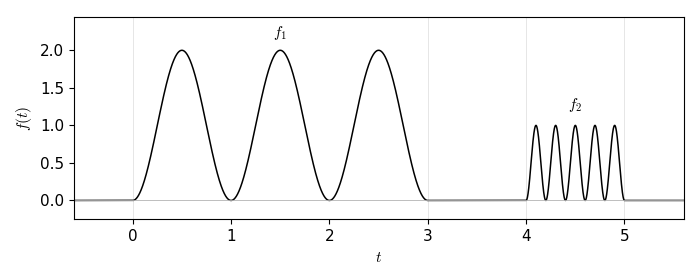
\includegraphics[width=0.9\textwidth]{abb1_signal.png}
  \caption{Das Signal $f$ aus Beispiel~\ref{bsp:testsignal}.} 
    %Links die
    %langsame Komponente auf $[0,3]$ mit Amplitude $2$, rechts die schnelle
    %auf $[4,5]$ mit Amplitude $1$.}
  \label{abb:signal}
\end{figure}

%An den vier Trägerrändern verschwinden $f$ und $f'$ gemeinsam, denn mit
%$1-\cos x = 2\sin^2(x/2)$ liegen dort doppelte Nullstellen. Das Signal ist
%also stetig differenzierbar; in Abbildung~\ref{abb:signal} sieht man, dass
%die Kurve tangential in die Nulllinie einläuft und keine Ecke bildet.

Zum Vergleich berechnen wir zuerst $\hat f$. In der Konvention aus
Bemerkung~\ref{bem:fourier-konvention} ist
\[
  \hat f(\omega)
  =\frac{1}{\sqrt{2\pi}}\int_{\R} f(t)e^{-i\omega t}\,dt
  =\frac{1}{\sqrt{2\pi}}\left(
      \int_0^3\bigl(1-\cos(2\pi t)\bigr)e^{-i\omega t}\,dt
      +\frac12\int_4^5\bigl(1-\cos(10\pi t)\bigr)e^{-i\omega t}\,dt
    \right).
\]

Wir behandeln beide Summanden getrennt und benutzen durchweg nur
\begin{equation}\label{eq:stammfunktion-exp}
  \int_\alpha^\beta e^{ct}\,dt=\frac{1}{c}\bigl(e^{c\beta}-e^{c\alpha}\bigr),
  \qquad c\in\mathbb{C}\setminus\{0\},
\end{equation}
sowie $\cos x=\tfrac12\bigl(e^{ix}+e^{-ix}\bigr)$.

\paragraph{Die langsame Komponente.}
Wir schreiben $q_1:=1-e^{-3i\omega}$ und zerlegen
\[
  \int_0^3\bigl(1-\cos(2\pi t)\bigr)e^{-i\omega t}\,dt
  =\underbrace{\int_0^3 e^{-i\omega t}\,dt}_{=:A_1}
   -\underbrace{\int_0^3 \cos(2\pi t)\,e^{-i\omega t}\,dt}_{=:B_1}.
\]
Nach \eqref{eq:stammfunktion-exp} mit $c=-i\omega$ ist
\[
  A_1=\frac{e^{-3i\omega}-1}{-i\omega}=\frac{q_1}{i\omega}.
\]
Für $B_1$ ersetzen wir den Cosinus und fassen die Exponenten zusammen:
\[
  \cos(2\pi t)e^{-i\omega t}
  =\tfrac12\Bigl(e^{i(2\pi-\omega)t}+e^{-i(2\pi+\omega)t}\Bigr),
\]
also nach \eqref{eq:stammfunktion-exp}
\[
  B_1=\frac{e^{i(2\pi-\omega)3}-1}{2i(2\pi-\omega)}
     +\frac{e^{-i(2\pi+\omega)3}-1}{-2i(2\pi+\omega)}.
\]
Hier greift die Wahl der Zahlen: wegen
\[
  e^{\pm i(2\pi\mp\omega)3}=e^{\pm 6\pi i}\,e^{-3i\omega}=e^{-3i\omega},
  \qquad\text{da } e^{\pm 6\pi i}=1,
\]
werden beide Zähler zu $\pm q_1$, und $q_1$ lässt sich ausklammern:
\[
  B_1=\frac{q_1}{2i}\left(\frac{1}{2\pi+\omega}-\frac{1}{2\pi-\omega}\right)
     =\frac{q_1}{2i}\cdot\frac{2\omega}{\omega^2-4\pi^2}
     =\frac{q_1\,\omega}{i\,(\omega^2-4\pi^2)}.
\]
Damit
\[
  A_1-B_1
  =\frac{q_1}{i}\left(\frac1\omega-\frac{\omega}{\omega^2-4\pi^2}\right)
  =\frac{q_1}{i}\cdot\frac{-4\pi^2}{\omega(\omega^2-4\pi^2)}
  =\frac{i\,4\pi^2\,q_1}{\omega\,(\omega^2-4\pi^2)} ,
\]
wobei im letzten Schritt $1/i=-i$ benutzt wurde.

\paragraph{Die schnelle Komponente.}
Dieselbe Rechnung mit $q_2:=e^{-4i\omega}-e^{-5i\omega}$ liefert
\[
  A_2=\int_4^5 e^{-i\omega t}\,dt=\frac{q_2}{i\omega},
  \qquad
  B_2=\frac{q_2\,\omega}{i\,(\omega^2-100\pi^2)} .
\]
Der entscheidende Schritt geht wieder auf, denn an beiden Integrations\-grenzen
ist $e^{10\pi i\cdot 4}=e^{40\pi i}=1$ und $e^{10\pi i\cdot 5}=e^{50\pi i}=1$.
Mit dem Amplitudenfaktor $\tfrac12$ folgt
\[
  \frac12\bigl(A_2-B_2\bigr)=\frac{i\,50\pi^2\,q_2}{\omega\,(\omega^2-100\pi^2)} .
\]

\paragraph{Ergebnis.}
Zusammensetzen und den Vorfaktor zurückholen:
\begin{equation}\label{eq:ft-testsignal}
  \hat f(\omega)
  =\frac{i}{\sqrt{2\pi}\,\omega}
   \left[
     \frac{4\pi^{2}\bigl(1-e^{-3i\omega}\bigr)}{\omega^{2}-4\pi^{2}}
     +\frac{50\pi^{2}\bigl(e^{-4i\omega}-e^{-5i\omega}\bigr)}{\omega^{2}-100\pi^{2}}
   \right].
\end{equation}

\anmerkung{In den Zählern stehen ausschließlich die Trägerränder: $0$ und
$3$ in $1-e^{-3i\omega}$, $4$ und $5$ in $e^{-4i\omega}-e^{-5i\omega}$.
Die Lageinformation steckt also vollständig in vier Phasenfaktoren, die
Frequenzinformation in den Nennern $\omega^2-(2\pi)^2$ und
$\omega^2-(10\pi)^2$.}

Die Nullstellen der Nenner bei $\omega\in\{0,\pm2\pi,\pm10\pi\}$ sind
hebbar, da dort auch die Zähler verschwinden: für $\omega=2\pi$ etwa ist
$e^{-3i\cdot 2\pi}=1$, also $q_1=0$. Die Grenzwerte sind
\[
  |\hat f(0)|=\frac{7}{2\sqrt{2\pi}}\approx 1{,}396,\qquad
  |\hat f(\pm2\pi)|=\frac{3}{2\sqrt{2\pi}}\approx 0{,}598,\qquad
  |\hat f(\pm10\pi)|=\frac{1}{4\sqrt{2\pi}}\approx 0{,}0997 .
\]

\begin{figure}[htbp]
  \centering
  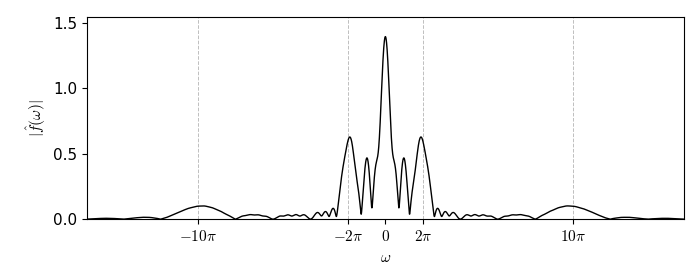
\includegraphics[width=0.9\textwidth]{abb2_fourier.png}
  \caption{Betragsspektrum $|\hat f(\omega)|$ nach \eqref{eq:ft-testsignal};
    gestrichelt die Stellen $\pm2\pi$ und $\pm10\pi$.}
  \label{abb:fourier}
\end{figure}

Abbildung~\ref{abb:fourier} zeigt beide Frequenzen als Maxima an den
erwarteten Stellen. %Zwei Beobachtungen sind wesentlich.

%Erstens ist der Ausschlag bei $\pm10\pi$ mit $0{,}0997$ auf etwa sieben
%Prozent des Maximums bei $\omega=0$ zusammengeschrumpft und von den
%Nebenmaxima der langsamen Komponente kaum zu unterscheiden. Der Grund ist
%die kurze Dauer: die schnelle Schwingung ist nur ein Viertel so lange
%aktiv wie die langsame und trägt entsprechend wenig zum Integral bei.

$|\hat f|$ enthält keine Auskunft darüber, wann die jeweilige Frequenz
auftritt. Vertauschte man die beiden Komponenten auf der Zeitachse, so
änderte sich nach \eqref{eq:ft-testsignal} nur die Phase, das Bild bliebe
dasselbe. Die zeitliche Information ist zwar in $\hat f$ vorhanden, aber
im Betragsspektrum unzugänglich.

Wir transformieren nun mit dem Haar-Wavelet $\psi^{\mathrm H}$ aus
Beispiel~\ref{bsp:haar} und beschränken uns auf $a>0$. Da
$\psi^{\mathrm H}$ reellwertig ist, entfällt die Konjugation in der
Definition:
\[
  W_{\psi^{\mathrm H}}f(a,b)
  =\frac{1}{\sqrt a}\int_{\R} f(t)\,
    \psi^{\mathrm H}\!\left(\frac{t-b}{a}\right)dt .
\]

Zunächst schreiben wir die verschobene und skalierte Version explizit hin.
Auflösen der drei definierenden Ungleichungen nach $t$ ergibt
\[
  \psi^{\mathrm H}\!\left(\frac{t-b}{a}\right)=
  \begin{cases}
     1, & b\le t< b+\tfrac a2,\\
    -1, & b+\tfrac a2\le t< b+a,\\
     0, & \text{sonst}.
  \end{cases}
\]
%etwa wird aus $0\le\frac{t-b}{a}<\tfrac12$ durch Multiplikation mit $a>0$
%und Addition von $b$ die Bedingung $b\le t<b+\tfrac a2$. 
Das Wavelet ist
also ein Fenster über $[b,\,b+a]$: die Verschiebung $b$ legt fest,
wo es sitzt, die Skala $a$, wie breit es ist, und die
Sprungstelle liegt genau in der Mitte.

Da der Integrand außerhalb dieses Fensters verschwindet und dort nur die
Werte $\pm1$ annimmt, ist
\[
  W_{\psi^{\mathrm H}}f(a,b)
  =\frac{1}{\sqrt a}\left(\int_b^{b+a/2} f(t)\,dt-\int_{b+a/2}^{b+a} f(t)\,dt\right).
\]
Die Transformation vergleicht den Mittelwert von $f$ auf der linken
Fensterhälfte mit dem auf der rechten; sie wirkt als Differenzenfilter.

Mit der Stammfunktion $F(t):=\int_{-\infty}^{t}f(s)\,ds$ wird daraus
\begin{equation}\label{eq:cwt-haar-exakt}
  W_{\psi^{\mathrm H}}f(a,b)
  =\frac{\bigl(F(b+\tfrac a2)-F(b)\bigr)-\bigl(F(b+a)-F(b+\tfrac a2)\bigr)}{\sqrt a}
  =\frac{2F\bigl(b+\tfrac a2\bigr)-F(b)-F(b+a)}{\sqrt a}.
\end{equation}
%Bemerkenswert daran ist, dass keine Fallunterscheidung nötig wird: hätte
%man stattdessen nach dem Träger von $f$ zerlegt, wären über ein Dutzend
%Lagen von $[b,b+a]$ relativ zu $[0,3]$ und $[4,5]$ zu behandeln.

Die Stammfunktion lässt sich explizit angeben. Es gilt
\[
  F(t)=
  \begin{cases}
    0, & t<0,\\
    t-\dfrac{\sin(2\pi t)}{2\pi}, & 0\le t\le 3,\\
    3, & 3\le t\le 4,\\
    3+\dfrac{t-4}{2}-\dfrac{\sin(10\pi t)}{20\pi}, & 4\le t\le 5,\\
    \dfrac72, & t>5.
  \end{cases}
\]

\anmerkung{ich hab die stammfkt jetzt einfach so gewählt dass sie steig ist?}
%Die Konstanten auf den beiden Plateaus sind $F(3)=3$ und $F(5)=\tfrac72$,
%denn $\sin(6\pi)=\sin(40\pi)=\sin(50\pi)=0$ -- zum zweiten und dritten Mal
%geht hier die ganzzahlige Periodenzahl ein. Insbesondere ist
%$F(t)=\int_\R f=\tfrac72$ für $t>5$, in Übereinstimmung mit
%$|\hat f(0)|=\tfrac{7}{2\sqrt{2\pi}}$.

Zeichnet man nun $W_{\psi^{\mathrm H}}f(a,b)$ als Funktion von $b$ und $a$, so ergibt sich Abbildung~\ref{abb:cwt}. Die Skalenachse ist logarithmisch,
um die große Spannweite von $a$ übersichtlich darzustellen.

\begin{figure}[htbp]
  \centering
  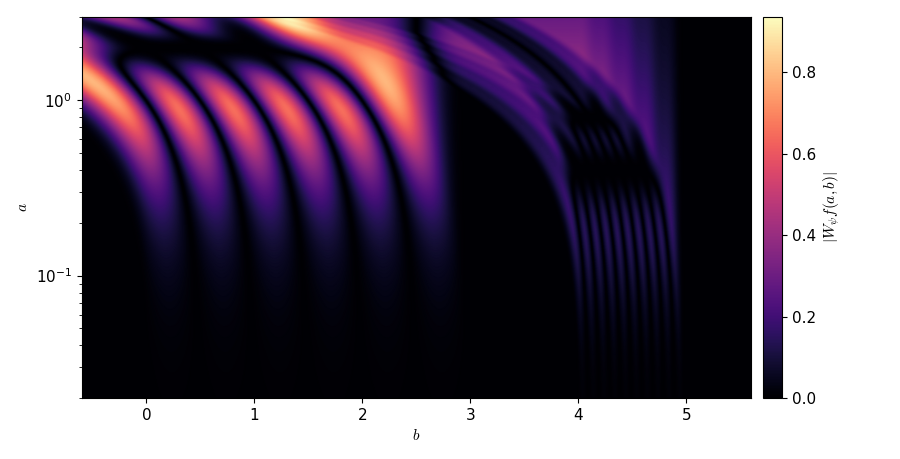
\includegraphics[width=\textwidth]{abb3_cwt_haar.png}
  \caption{Betrag der Wavelet-Transformierten nach
    \eqref{eq:cwt-haar-exakt}; die Skalenachse ist logarithmisch.}
  \label{abb:cwt}
\end{figure}

Abbildung~\ref{abb:cwt} zerfällt in zwei Bereiche. In der Ortsvariablen
$b$ liegen sie über den Trägern $[0,3]$ und $[4,5]$, in der Skala $a$
unterscheiden sie sich um den Faktor fünf -- also um genau das Verhältnis
der beiden Frequenzen. Beide Informationen, Zeitpunkt und Frequenz, sind
gleichzeitig ablesbar. Das ist der Gewinn gegenüber
Abbildung~\ref{abb:fourier}.

Auch die schwache schnelle Komponente, die im Fourier-Bild fast
verschwand, ist hier deutlich als eigenes Band zu erkennen. Der Grund ist,
dass die Transformation bei kleinem $a$ nur ein kurzes Zeitfenster
auswertet und die lange Dauer der langsamen Komponente dort nicht mehr ins
Gewicht fällt.

\end{Beispiel}

\anmerkung{Die Bänder sind auffällig breit. Das liegt am
Abklingverhalten $|\hat\psi^{\mathrm H}(\omega)|=O(|\omega|^{-1})$: das
Haar-Wavelet ist im Zeitbereich perfekt, im Frequenzbereich aber nur
schwach lokalisiert. Diese Asymmetrie motiviert die Konstruktion glatterer
Wavelets in Kapitel~4.}

\anmerkung{Die Streifen kippen mit wachsendem $a$ nach links, weil
$\operatorname{supp}\psi^{\mathrm H}_{a,b}=[b,\,b+a]$ rechts von $b$ liegt
und nicht symmetrisch um $b$. Das ist kein Artefakt, sondern eine
Eigenschaft der in Beispiel~\ref{bsp:haar} gewählten Normierung.}

Damit ist an einem Beispiel vorgeführt, was die Transformation leistet:
sie trennt, was im Betragsspektrum vermengt bleibt. Offen ist bislang, ob
sich $f$ aus $W_\psi f$ zurückgewinnen lässt.

\quellen{Haar-Wavelet und seine Fourier-Transformierte:
\cite[Kap.~1.1]{lmr}, \cite[Kap.~1.6]{blatter}. Zur Darstellung von
Wavelet-Transformierten und zur Wahl zusammengesetzter Testsignale
vgl.\ \cite[Kap.~3.1]{blatter} sowie \cite[Kap.~1.1]{lmr}.}

%\anmerkung{AUSGELAGERT (Block~A3, ca.\ acht Seiten): die affinen Operatoren $D_a$ und
%$T_b$ mit Unitaritätsbeweis, das Verknüpfungsgesetz und die Nichtkommutativität der
%affinen Gruppe, der Kovarianzsatz, die Fourier-Darstellung der CWT und die
%Filterdarstellung als Faltung samt Bandpasscharakter. Sachlich richtig und sauber
%bewiesen, aber keiner dieser Sätze wird in Kapitel~\ref{chapter:dwt} oder
%\ref{chapter:denoising} noch einmal gebraucht. Die inhaltliche Substanz ist unten in
%zwei Absätze zusammengezogen.}

%\subsubsection*{Die CWT als Filterbank}
%
%Bei festgehaltener Skala ist die CWT eine Faltung. Setzt man
%$\psi^{-}_{a}(u) := \lvert a\rvert^{-1/2}\,\psi(-u/a)$, so ist
%$W_\psi f(a,\cdot) = f * \psi^{-}_{a}$ und folglich
%\[
%  \bigl(W_\psi f(a,\cdot)\bigr)^{\wedge}(\omega)
%  \;=\; (2\pi)^{1/2}\,\lvert a\rvert^{1/2}\,\hat\psi(a\omega)\,\hat f(\omega).
%\]
%Die CWT ist bei festem $a$ also ein linearer, zeitinvarianter Filter mit
%Übertragungsfunktion $H_a(\omega) = (2\pi)^{1/2}\lvert a\rvert^{1/2}\hat\psi(a\omega)$.
%Wegen $\hat\psi(0) = 0$ nach Satz~\ref{satz:zulaessigkeit-mittelwert} und
%$\hat\psi(\omega)\to 0$ für $\lvert\omega\rvert\to\infty$ (Riemann--Lebesgue) ist jedes
%$H_a$ ein Bandpass. Ist $\lvert\hat\psi\rvert$ um eine Frequenz $\omega_0>0$ mit Breite
%$\Delta$ konzentriert, so liegt das Durchlassband bei allgemeinem $a$ um
%$\omega_0/\lvert a\rvert$ und hat die Breite $\Delta/\lvert a\rvert$; das Verhältnis von
%Mittenfrequenz zu Bandbreite ist damit von $a$ unabhängig. Die Skalenachse entspricht
%einer Filterbank mit \emph{konstanter relativer} Bandbreite -- im Unterschied zur
%konstanten \emph{absoluten} Bandbreite der gefensterten Fourier-Transformation.
%
%\quellen{LMR, Kap.~1.3 Filtereigenschaften der Wavelet-Transformation, S.~28--30,
%insbesondere Lemma~1.3.1, S.~29 \cite[S.~28--30]{lmr}; Blatter, Kap.~3.1,
%Gl.~(8)--(10), S.~56--57 \cite[S.~56--57]{blatter}.}
%
%\begin{Bemerkung}[Bedeutung für das EKG]
%\label{bem:filter-ekg}
%Die Filterdarstellung erklärt, weshalb die Wavelet-Analyse für
%EKG-Signale strukturell passend ist. Der QRS-Komplex ist ein Transient mit
%steilen Flanken und daher breitbandig mit Schwerpunkt bei hohen Frequenzen; er
%erscheint in $W_\psi f(a,\cdot)$ bei kleinen $\lvert a\rvert$. P- und T-Welle
%sind niederfrequent und erscheinen bei großen $\lvert a\rvert$. Da die
%Bandbreite mit $1/\lvert a\rvert$ mitwächst, wird der QRS-Komplex zeitlich
%scharf lokalisiert, während die T-Welle mit hinreichender Frequenzauflösung
%erfasst wird -- beides mit demselben Werkzeug. Da $\hat\psi(0) = 0$ ist,
%unterdrückt zudem jeder Filter $H_a$ den Gleichanteil; die für EKG-Aufzeichnungen
%typische Basisliniendrift wirkt sich daher nur auf die gröbsten Skalen aus.
%\end{Bemerkung}
% 
%\quellen{Zum klinischen Frequenzgehalt der EKG-Komponenten: Gacek
%\cite{gacek}; Chatterjee et al., Abschnitt~2 \cite{chatterjee}; Aqil, Kap.~1--2,
%S.~51--55 \cite[S.~51--55]{aqil}.}
% 
%\anmerkung{Seitenzahlen für Gacek und Chatterjee bitte noch ergänzen --
%diese Bemerkung ist die inhaltliche Brücke zu Kapitel~\ref{chapter:anwendung} und
%sollte belegt sein.}
 
% ============================================================
 
\subsection{Die Plancherel-Formel}
\label{subsec:plancherel}
 
Die CWT bildet eine Funktion einer Variablen auf eine Funktion zweier Variablen
ab. Damit sich überhaupt von einer Isometrie sprechen lässt, ist auf der
Bildseite ein Hilbertraum zu wählen -- und zwar nicht mit dem Lebesgue-Maß
$da\,db$, sondern mit dem gewichteten Maß $\lvert a\rvert^{-2}\,da\,db$. Dass
gerade dieses Gewicht die Isometrie erzwingt, ist keine Willkür: Jede andere
Potenz erzeugte in der Rechnung einen frequenzabhängigen Restfaktor.
 
\begin{Definition}[Bildraum]
\label{def:bildraum}
Auf $\R^*_\square = \R^*\times\R$ sei das Maß
$d\mu(a,b) = \lvert a\rvert^{-2}\,da\,db$ zugrunde gelegt und
\[
  \mathcal H \;:=\; L^2\bigl(\R^*_\square,\, d\mu\bigr),
  \qquad
  \scal{u}{v}_{\mathcal H} \;:=\; \int_{\R^*_\square} u(a,b)\,\overline{v(a,b)}\;\frac{da\,db}{a^2} .
\]
\end{Definition}
 
\quellen{Blatter, Kap.~3.2, S.~61--62 \cite[S.~61--62]{blatter}.}
 
\begin{Satz}[Plancherel-Formel für die CWT]
\label{satz:plancherel-cwt}
Sei $\psi$ ein Wavelet mit Zulässigkeitskonstante $C_\psi$ gemäß
\eqref{eq:zulaessigkeit}. Dann ist $W_\psi f \in \mathcal H$ für jedes
$f \in \LZwei$, und es gilt
\begin{equation}
\label{eq:plancherel-cwt}
  \scal{W_\psi f}{W_\psi g}_{\mathcal H} \;=\; C_\psi\,\scal{f}{g}
  \qquad\text{für alle } f,g \in \LZwei .
\end{equation}
Insbesondere ist $C_\psi^{-1/2}\,W_\psi \colon \LZwei \to \mathcal H$ eine
Isometrie; $W_\psi$ ist injektiv und besitzt abgeschlossenes Bild.
\end{Satz}
 

\quellen{Blatter, Satz~(3.3) mit Beweis, S.~62--63 \cite[S.~62--63]{blatter};
LMR, Satz~1.1.8 mit Lemma~1.1.7, S.~22--23 \cite[S.~22--23]{lmr}.}

\anmerkung{AUSGELAGERT (Block~A4): der vierschrittige Beweis (Tonelli --
Identifikation der inneren Integrale -- Zusammensetzen -- Polarisation), die Bemerkung
zur Notwendigkeit des Gewichts $\lvert a\rvert^{-2}$, die Halbebenen-Variante und der
Fall zweier verschiedener Wavelets. Der Beweis ist die stärkste eigene Leistung des
alten Kapitels~3 -- er korrigiert eine Vertauschungslücke bei Blatter. Wenn Du an
\emph{einer} Stelle im CWT-Teil doch einen vollen Beweis führen willst, dann hier.
Kostet gut zwei Seiten.}

\begin{Bemerkung}[Redundanz -- und warum die CWT nicht das letzte Wort sein kann]
\label{bem:redundanz}
Satz~\ref{satz:plancherel-cwt} sichert die Umkehrbarkeit, macht zugleich aber das
Grundproblem sichtbar: Die CWT bildet eine Funktion \emph{einer} Variablen auf eine
Funktion \emph{zweier} Variablen ab. Ihr Bild $W_\psi(\LZwei)$ ist deshalb nur ein
echter abgeschlossener Teilraum von $\mathcal H$; die Werte $W_\psi f(a,b)$ sind
untereinander gekoppelt und tragen in hohem Maße redundante Information. Für eine
numerische Verarbeitung -- und erst recht für die Statistik in
Kapitel~\ref{chapter:denoising} -- ist das untauglich: Dort wird eine
\emph{Orthonormalbasis} gebraucht, denn nur unter einer unitären Abbildung bleibt die
Statistik des Rauschens erhalten. Gesucht ist also eine abzählbare Teilmenge von
Parametern $(a,b)$, aus der sich $f$ noch vollständig rekonstruieren lässt und für die
das System $\{\psi_{a,b}\}$ orthonormal ist. Der Rest dieses Kapitels führt dorthin.
\end{Bemerkung}

\anmerkung{Diese Bemerkung ersetzt den gestrichenen Abschnitt über Frames und
Rieszbasen. Frames sind der allgemeinere Rahmen (stabile, aber überbestimmte
Darstellungen); für diese Arbeit werden sie nicht gebraucht, weil die MSA direkt eine
Orthonormalbasis liefert. Belege, falls Du den Abschnitt doch wieder aufnimmst:
LMR, Kap.~2.1, S.~87--109; Blatter, Kap.~4.1--4.2, S.~79--90.}

%%%%%%%%%%%%%%%%%%%%%%%%%%%%%%%%%%%%%%%%%%%%%%%%%%%%%%%%%%%%%%%%%%%%%%%%%%%%%%%
\section{Das dyadische Gitter und die Multiskalenanalyse}
\label{sec:mra-axiome}
%%%%%%%%%%%%%%%%%%%%%%%%%%%%%%%%%%%%%%%%%%%%%%%%%%%%%%%%%%%%%%%%%%%%%%%%%%%%%%%

Nach Bemerkung~\ref{bem:redundanz} ist eine abzählbare Auswahl von Parametern
$(a,b)$ zu treffen. Welche Auswahl die richtige ist, sagt bereits das
Skalierungsverhalten der Transformation: Eine Stauchung des Signals verschiebt
die Transformierte entlang der $a$-Achse, und diese Verschiebung wird erst in
logarithmischen Koordinaten $\alpha = \log_2\lvert a\rvert$ zu einer
gleichmäßigen. Ein arithmetisches Skalengitter $a \in \{1,2,3,\dots\}$ würde die
feinen Skalen zu grob und die groben zu fein abtasten; ein geometrisches Gitter
$a = a_0^{\,j}$ mit festem $a_0 > 1$ tastet dagegen jede Oktave gleich dicht ab.

Für die Translationen folgt daraus unmittelbar die zweite Festlegung. Auf der
Skala $a = a_0^{\,j}$ hat das Analysefenster die Breite $a_0^{\,j}\cdot\lvert\supp\psi\rvert$.
Ein über alle Skalen \emph{fester} Translationsschritt $b_0$ wäre auf groben
Skalen redundant und auf feinen zu grob; der Schritt muss vielmehr mit der
Fensterbreite mitwachsen. Das führt auf $b = k\,b_0\,a_0^{\,j}$ mit $k \in \Z$.

\begin{Definition}[Dyadisches Gitter und diskrete Wavelet-Familie]
\label{def:dyadisch}
Sei $\psi$ ein Wavelet. Zu $a_0 > 1$ und $b_0 > 0$ heißt
\[
  \Gamma_{a_0,b_0} \;:=\; \bigl\{ (a_0^{\,j},\; k\,b_0\,a_0^{\,j}) \;:\; j,k \in \Z \bigr\}
  \;\subset\; \R^*_\square
\]
das zugehörige Skalengitter. Im \emph{dyadischen} Fall $a_0 = 2$, $b_0 = 1$
schreiben wir für die Elemente der Wavelet-Familie \eqref{eq:wavelet-familie}
kurz
\begin{equation}
\label{eq:dyadische-familie}
  \psi_{j,k} \;:=\; \psi_{2^{j},\,k2^{j}},
  \qquad\text{also}\qquad
  \psi_{j,k}(t) \;=\; 2^{-j/2}\,\psi\!\left(\frac{t}{2^{j}} - k\right),
  \qquad j,k \in \Z .
\end{equation}
\end{Definition}

\quellen{LMR, Definition~2.1.1, S.~88 \cite[S.~88]{lmr} (dort mit allgemeinen
Gitterparametern $a_0 > 1$, $b_0 > 0$; der dyadische Fall ist der Spezialfall
$a_0 = 2$); Blatter, Kap.~4.3, S.~91--99 \cite[S.~91--99]{blatter}; die
Schreibweise \eqref{eq:dyadische-familie} nach Blatter, S.~106
\cite[S.~106]{blatter} und LMR, Gl.~(2.2.6), S.~112 \cite[S.~112]{lmr}.}

\begin{Bemerkung}[Zur Indexkonvention]
\label{bem:indexkonvention}
In \eqref{eq:dyadische-familie} gehört zu \emph{kleinerem} $j$ die
\emph{feinere} Skala: Für $j \to -\infty$ ist $2^{j} \to 0$, das Wavelet
$\psi_{j,k}$ wird schmal und tastet kurze Transienten ab; für $j \to +\infty$
wird es breit. Diese Konvention wird in der gesamten Arbeit durchgehalten. Sie
stimmt mit Blatter und mit Louis/Maaß/Rieder überein, die beide die Kette
$\cdots \subset V_1 \subset V_0 \subset V_{-1} \subset \cdots$ mit
absteigendem Index für aufsteigende Feinheit schreiben. Blatter weist an der
entsprechenden Stelle ausdrücklich darauf hin, dass ein Teil der Literatur
genau umgekehrt zählt; Hanke-Bourgeois etwa arbeitet in $L^2(0,1)$ mit
aufsteigendem Index für zunehmende Feinheit. Bei Vergleichen mit dieser Quelle
ist der Index also zu spiegeln.
\end{Bemerkung}

\quellen{Blatter, S.~106 \cite[S.~106]{blatter} (dort der ausdrückliche
Warnhinweis, dass verschiedene Autoren umgekehrt nummerieren); LMR,
Definition~2.2.1, S.~111 \cite[S.~111]{lmr}; Hanke-Bourgeois, §56,
S.~434--435 \cite[S.~434--435]{hankebourgeois} mit der entgegengesetzten
Konvention.}

\begin{Bemerkung}[Kritische Abtastung]
\label{bem:kritische-abtastung}
Die Wahl $a_0 = 2$, $b_0 = 1$ ist die gröbste Diskretisierung, bei der noch
keine Information verlorengeht. Anschaulich: Auf der Skala $j$ liefert
\eqref{eq:dyadische-familie} genau einen Koeffizienten pro Zeitintervall der
Länge $2^{j}$, insgesamt also über alle Skalen hinweg
$\sum_{j} 2^{-j}$ Koeffizienten pro Zeiteinheit -- bei Beschränkung auf
$j \ge j_0$ gerade $2^{-j_0+1}$, das heißt in der Größenordnung der
Abtastrate des Signals selbst. Die Redundanz der CWT wird damit exakt auf null
reduziert. Feinere Gitter ($a_0 < 2$ oder $b_0 < 1$) führen auf überbestimmte,
aber stabile Darstellungen; deren allgemeine Theorie ist die der Frames und
wird hier nicht benötigt, da die Multiskalenanalyse den Orthonormalfall direkt
liefert.
\end{Bemerkung}

\quellen{LMR, Kap.~2.1, S.~87--109 \cite[S.~87--109]{lmr}; Blatter,
Kap.~4.1--4.3, S.~79--99 \cite[S.~79--99]{blatter}.}

\anmerkung{Hier bewusst nur anschaulich argumentiert („ein Koeffizient pro
Zelle``). Der präzise Begriff wäre das straffe Frame mit $A = B = 1$; das würde
den gestrichenen Frame-Abschnitt zurückholen. Für die Arbeit genügt, dass die
MSA am Ende eine Orthonormalbasis liefert -- das ist stärker als jede
Frame-Aussage.}

\subsection{Die Axiome}
\label{subsec:mra-axiome}

Die entscheidende Idee ist nun, das Wavelet nicht direkt zu suchen, sondern
zunächst die \emph{Approximationsräume} zu axiomatisieren, in denen die
Näherungen des Signals auf den einzelnen Skalen leben. Das Wavelet entsteht
danach als dasjenige Objekt, das den Übergang zwischen zwei benachbarten Skalen
beschreibt.

\begin{Definition}[Dilatationsoperator]
\label{def:dilatation}
Für $a \in \R^*$ sei $D_a \colon \LZwei \to \LZwei$, $(D_a f)(t) := \lvert a\rvert^{-1/2} f(t/a)$.
Die Substitution $t = as$ zeigt $\norm{D_a f}_{\LZwei} = \norm{f}_{\LZwei}$;
wegen $D_{1/a} D_a = \mathrm{id}$ ist $D_a$ unitär mit $D_a^{-1} = D_a^* = D_{1/a}$.
\end{Definition}

\quellen{LMR, Kap.~1.2 Affine Operatoren, Lemma~1.2.1, S.~26--27
\cite[S.~27]{lmr}; Blatter, Kap.~3.2, S.~61 \cite[S.~61]{blatter}.}

\begin{Definition}[Multiskalenanalyse]
\label{def:msa}
Eine \emph{Multiskalenanalyse} (MSA) von $\LZwei$ ist eine Folge
$(V_j)_{j\in\Z}$ abgeschlossener Teilräume von $\LZwei$ mit den folgenden
Eigenschaften:
\begin{enumerate}
\item[(M1)] \emph{(Schachtelung)}
  $\;\cdots \subset V_{2} \subset V_{1} \subset V_{0} \subset V_{-1} \subset V_{-2} \subset \cdots \subset \LZwei$,
\item[(M2)] \emph{(Separation)}
  $\;\displaystyle\bigcap_{j\in\Z} V_j = \{0\}$,
\item[(M3)] \emph{(Vollständigkeit)}
  $\;\displaystyle\overline{\bigcup_{j\in\Z} V_j} = \LZwei$,
\item[(M4)] \emph{(Skalierung)}
  $\;V_{j+1} = D_2(V_j)$ für alle $j \in \Z$, gleichbedeutend mit
  $f \in V_j \iff f(2^{j}\,\cdot\,) \in V_0$,
\item[(M5)] \emph{(Erzeugende Funktion)} Es gibt ein
  $\varphi \in \LZwei \cap L^1(\R)$, sodass $\{\varphi(\,\cdot - k) : k \in \Z\}$
  eine Orthonormalbasis von $V_0$ ist.
\end{enumerate}
Die Funktion $\varphi$ heißt \emph{Skalierungsfunktion} der MSA.
\end{Definition}

\quellen{Blatter, Kap.~5.1 Axiomatische Beschreibung, Bedingungen (a)--(c),
S.~106 \cite[S.~106]{blatter} -- die hier verwendete Fassung folgt Blatter,
insbesondere in der Forderung einer Orthonormalbasis in (M5); LMR,
Definition~2.2.1 mit (2.2.2)--(2.2.5), S.~111 \cite[S.~111]{lmr}.}

\begin{Bemerkung}[Zu den Axiomen]
\label{bem:msa-axiome}
\begin{enumerate}
\item[(a)] Die anschauliche Bedeutung von (M1)--(M3): Ein $f \in V_j$ enthält
  nur Strukturen der zeitlichen Ausdehnung $\gtrsim 2^{j}$. Je kleiner $j$,
  desto feinere Details sind zugelassen; (M3) besagt, dass im Limes
  $j \to -\infty$ jedes Signal erreichbar ist, (M2), dass im Limes
  $j \to +\infty$ nichts übrigbleibt.
\item[(b)] Axiom (M4) ist die eigentliche Substanz: Die $V_j$ sind nicht
  irgendwelche geschachtelten Räume, sondern skalierte Kopien ein und desselben
  Raumes $V_0$. Erst dadurch genügt \emph{eine} Funktion $\varphi$, um die
  gesamte Hierarchie festzulegen.
\item[(c)] LMR fordern in (M5) statt einer Orthonormalbasis nur eine
  Riesz-Basis, also die Existenz von Konstanten $0 < A \le B$ mit
  $A\sum_k \lvert c_k\rvert^2 \le \bigl\lVert \sum_k c_k \varphi(\,\cdot-k)\bigr\rVert^2_{\LZwei} \le B\sum_k\lvert c_k\rvert^2$.
  Das ist die allgemeinere Formulierung; aus jeder Riesz-Basis lässt sich durch
  einen Orthogonalisierungsschritt im Fourier-Bereich eine Orthonormalbasis
  desselben Raumes gewinnen, die weiterhin aus ganzzahligen Translaten einer
  einzigen Funktion besteht. Da die Arbeit die Orthonormalität ohnehin benötigt,
  wird sie hier gleich gefordert.
\item[(d)] Die Zusatzforderung $\varphi \in L^1(\R)$ in (M5) folgt Blatter und
  sichert, dass $\hat\varphi$ stetig ist -- das wird in
  Kapitel~\ref{chapter:dwt} bei der Auswertung der Skalierungsgleichung an der
  Stelle $\omega = 0$ gebraucht.
\end{enumerate}
\end{Bemerkung}

\quellen{LMR, Bemerkung~2.2.2, S.~112--113 \cite[S.~112--113]{lmr}
(Interpretation der Grenzübergänge und Translationsinvarianz); zum
Orthogonalisierungstrick Blatter, Kap.~5.2, S.~110 \cite[S.~110]{blatter} und
LMR, Satz~2.2.5, S.~115 \cite[S.~115]{lmr} [geschätzt].}

\anmerkung{Die Seitenzahl für LMR Satz 2.2.5 ist geschätzt -- der Satz liegt im
Abschnitt 2.2.1 (S.~110--127), die genaue Seite habe ich nicht verifiziert. Vor
der Abgabe nachschlagen oder den Verweis streichen.}

\begin{Beispiel}[Die Haar-MSA]
\label{bsp:haar-msa}
Sei $\varphi := \mathbf{1}_{[0,1[}$ und
\[
  V_0 \;:=\; \bigl\{ f \in \LZwei : f \text{ ist konstant auf } [k,k+1[ \text{ für alle } k \in \Z \bigr\},
  \qquad V_j := D_{2^{j}}(V_0).
\]
Dann ist $V_j$ der Raum der Treppenfunktionen mit Sprungstellen in $2^{j}\Z$,
und (M1) sowie (M4) sind unmittelbar klar. Die Translate
$\{\varphi(\,\cdot-k)\}$ haben paarweise disjunkte Träger und die Norm $1$,
bilden also eine Orthonormalbasis von $V_0$, womit (M5) gilt. Die Separation
(M2) ist trivial: Eine Funktion, die für jedes $j$ auf Intervallen der Länge
$2^{j}$ konstant ist, ist konstant auf $\R$ und als Element von $\LZwei$ dann
null. Die Vollständigkeit (M3) folgt daraus, dass die Treppenfunktionen mit
dyadisch rationalen Sprungstellen dicht in $\LZwei$ liegen.
\end{Beispiel}

\quellen{Blatter, Kap.~5.1, Beispiel~$\textcircled{1}$, S.~107
\cite[S.~107]{blatter}; LMR, Beispiel zu Kap.~2.2.1, S.~113
\cite[S.~113]{lmr}; Hanke-Bourgeois, §56, Gl.~(56.1)--(56.2), S.~434--435
\cite[S.~434--435]{hankebourgeois} (dort in $L^2(0,1)$ und mit gespiegeltem
Index, vgl.\ Bemerkung~\ref{bem:indexkonvention}).}

\anmerkung{Dieses Beispiel wird in Kapitel~\ref{chapter:dwt} bis zum
Haar-Wavelet durchgerechnet und ist in Kapitel~\ref{chapter:anwendung} der
Referenzfall, gegen den \texttt{db2} antritt. Es lohnt sich, es hier vollständig
zu bringen.}

%%%%%%%%%%%%%%%%%%%%%%%%%%%%%%%%%%%%%%%%%%%%%%%%%%%%%%%%%%%%%%%%%%%%%%%%%%%%%%%
\section{Skalierungsfunktion und Orthonormalbasis der Räume \texorpdfstring{$V_j$}{Vj}}
\label{sec:skalierungsfunktion}
%%%%%%%%%%%%%%%%%%%%%%%%%%%%%%%%%%%%%%%%%%%%%%%%%%%%%%%%%%%%%%%%%%%%%%%%%%%%%%%

Axiom (M5) stattet nur den Grundraum $V_0$ mit einer Basis aus. Dass sich diese
auf alle Skalen vererbt, ist eine unmittelbare Folge von (M4) und der Unitarität
des Dilatationsoperators -- und damit derselbe Mechanismus, der schon in
Definition~\ref{def:cwt} den Normierungsfaktor $\lvert a\rvert^{-1/2}$ erzwungen
hat.

\begin{Satz}[Orthonormalbasis von $V_j$]
\label{satz:onb-vj}
Sei $(V_j)_{j\in\Z}$ eine MSA mit Skalierungsfunktion $\varphi$. Setzt man
\begin{equation}
\label{eq:phi-jk}
  \varphi_{j,k}(t) \;:=\; 2^{-j/2}\,\varphi\!\left(\frac{t}{2^{j}} - k\right),
  \qquad j,k \in \Z ,
\end{equation}
so ist $\{\varphi_{j,k} : k \in \Z\}$ für jedes feste $j$ eine Orthonormalbasis
von $V_j$.
\end{Satz}

\begin{proof}
Aus (M4) folgt durch Induktion $V_j = D_{2^{j}}(V_0)$ für alle $j \in \Z$.
Nach Definition~\ref{def:dilatation} ist $D_{2^{j}}$ ein unitärer Operator auf
$\LZwei$; unitäre Operatoren bilden Orthonormalbasen eines abgeschlossenen
Teilraums auf Orthonormalbasen des Bildraums ab, denn sie erhalten
Skalarprodukte und sind surjektiv auf das Bild. Nach (M5) ist
$\{\varphi(\,\cdot-k) : k\in\Z\}$ eine Orthonormalbasis von $V_0$, also ist
$\{D_{2^{j}}\varphi(\,\cdot-k) : k\in\Z\}$ eine Orthonormalbasis von $V_j$.
Es bleibt die Identifikation
\[
  \bigl(D_{2^{j}}\varphi(\,\cdot-k)\bigr)(t)
  \;=\; 2^{-j/2}\,\varphi\!\left(\frac{t}{2^{j}} - k\right)
  \;=\; \varphi_{j,k}(t),
\]
womit die Behauptung gezeigt ist.
\end{proof}

\quellen{Blatter, Kap.~5.1, S.~107 \cite[S.~107]{blatter} (dort ohne
ausgeführten Beweis: „Aus (b) folgt dann ohne weiteres\dots``); LMR, Gl.~(2.2.6)
und (2.2.7), S.~112 \cite[S.~112]{lmr}.}

\anmerkung{Der Beweis ist kurz, aber es lohnt, ihn zu führen: Er macht sichtbar,
dass die \emph{gesamte} Konstruktion an der Unitarität von $D_2$ hängt -- also
an genau derselben Eigenschaft, die in Abschnitt~\ref{sec:onb-invarianz} das
Rauschen invariant lässt. Das ist der rote Faden der Arbeit an einer Stelle, an
der man ihn sonst übersieht.}

\begin{Definition}[Approximationsoperator]
\label{def:projektion-pj}
Es bezeichne $P_j \colon \LZwei \to V_j$ die Orthogonalprojektion auf $V_j$.
Nach Satz~\ref{satz:onb-vj} gilt
\begin{equation}
\label{eq:pj}
  P_j f \;=\; \sum_{k\in\Z} \scal{f}{\varphi_{j,k}}\,\varphi_{j,k},
  \qquad f \in \LZwei .
\end{equation}
Die Zahlen $a_{j,k} := \scal{f}{\varphi_{j,k}}$ heißen
\emph{Approximationskoeffizienten} von $f$ auf der Skala $j$.
\end{Definition}

\quellen{Blatter, Kap.~5.1, Gl.~(7), S.~107 \cite[S.~107]{blatter}; LMR,
Bemerkung~2.2.2\,(a), S.~112 \cite[S.~112]{lmr}.}

\begin{Proposition}[Approximationseigenschaft]
\label{prop:approximation}
Für jedes $f \in \LZwei$ gilt
\[
  \lim_{j\to-\infty} \norm{P_j f - f}_{\LZwei} = 0
  \qquad\text{und}\qquad
  \lim_{j\to+\infty} \norm{P_j f}_{\LZwei} = 0 .
\]
\end{Proposition}

\begin{proof}
Für die erste Aussage sei $\varepsilon > 0$. Nach (M3) gibt es ein
$g \in \bigcup_{j} V_j$ mit $\norm{f-g}_{\LZwei} < \varepsilon$, etwa
$g \in V_{j_0}$. Für jedes $j \le j_0$ ist $V_{j_0} \subset V_j$ nach (M1), also
$g \in V_j$. Da $P_j f$ die Bestapproximation von $f$ in $V_j$ ist, folgt
\[
  \norm{f - P_j f}_{\LZwei} \;\le\; \norm{f-g}_{\LZwei} \;<\; \varepsilon
  \qquad\text{für alle } j \le j_0 .
\]
Die zweite Aussage beruht auf (M2) und wird hier zitiert.
\end{proof}

\quellen{LMR, Bemerkung~2.2.2\,(a), S.~112--113 \cite[S.~112--113]{lmr}
(beide Grenzübergänge, dort ohne Beweis formuliert); Blatter, Kap.~5.1,
S.~106 \cite[S.~106]{blatter}.}

\anmerkung{Die zweite Aussage ist deutlich unangenehmer als die erste -- aus
$\bigcap V_j = \{0\}$ allein folgt $\norm{P_j f} \to 0$ nicht ohne weiteres,
man braucht ein Argument über die monoton fallenden Normen und den Limes der
$P_j f$. Vorschlag: zitieren und nicht beweisen. Für die Arbeit wird nur die
erste Aussage wirklich gebraucht, nämlich in
Abschnitt~\ref{sec:duennbesetztheit}.}

\subsection{Die Orthonormalität im Fourier-Bereich}
\label{subsec:onb-fourier}

Für die Konstruktion in Kapitel~\ref{chapter:dwt} wird die Orthonormalität der
Translate nicht in der obigen Form, sondern als Bedingung an $\hat\varphi$
gebraucht. Die Übersetzung ist eine reine Fourier-Reihen-Rechnung und wird hier
gleich mitgenommen.

\begin{Lemma}[Orthonormalitätsbedingung]
\label{lem:onb-fourier}
Sei $\varphi \in \LZwei$. Dann sind äquivalent:
\begin{enumerate}
\item[(i)] $\{\varphi(\,\cdot-k) : k \in \Z\}$ ist ein Orthonormalsystem in $\LZwei$,
\item[(ii)] $\displaystyle\sum_{l\in\Z} \bigl\lvert \hat\varphi(\omega + 2\pi l)\bigr\rvert^{2}
  \;=\; \frac{1}{2\pi} \qquad\text{für fast alle } \omega \in \R .$
\end{enumerate}
\end{Lemma}

\begin{proof}
Nach dem Satz von Plancherel und der Rechenregel
$\bigl(\varphi(\,\cdot-k)\bigr)^{\wedge}(\omega) = e^{-ik\omega}\hat\varphi(\omega)$
ist
\[
  \scal{\varphi}{\varphi(\,\cdot-k)}
  \;=\; \scal{\hat\varphi}{e^{-ik\,\cdot}\hat\varphi}
  \;=\; \int_\R \lvert\hat\varphi(\omega)\rvert^{2}\, e^{ik\omega}\,d\omega .
\]
Wir zerlegen $\R$ in die Intervalle $[2\pi l, 2\pi(l+1)[$ und substituieren
$\omega \mapsto \omega + 2\pi l$. Da $e^{ik\omega}$ die Periode $2\pi$ hat,
liefert das
\[
  \scal{\varphi}{\varphi(\,\cdot-k)}
  \;=\; \int_0^{2\pi} \Phi(\omega)\, e^{ik\omega}\,d\omega,
  \qquad
  \Phi(\omega) := \sum_{l\in\Z}\bigl\lvert\hat\varphi(\omega+2\pi l)\bigr\rvert^{2} .
\]
Die Vertauschung von Summe und Integral ist nach dem Satz von Beppo Levi
zulässig, da alle Summanden nichtnegativ sind; insbesondere ist
$\Phi \in L^1(0,2\pi)$ mit
$\int_0^{2\pi}\Phi = \norm{\hat\varphi}^2_{\LZwei} = \norm{\varphi}^2_{\LZwei} < \infty$,
und $\Phi$ ist $2\pi$-periodisch.

Bezeichnet $c_k := (2\pi)^{-1}\int_0^{2\pi}\Phi(\omega)e^{ik\omega}\,d\omega$ den
$k$-ten Fourier-Koeffizienten von $\Phi$, so ist die Orthonormalität (i)
gleichbedeutend mit
\[
  2\pi\,c_k \;=\; \scal{\varphi}{\varphi(\,\cdot-k)} \;=\; \delta_{k,0}
  \qquad\text{für alle } k \in \Z,
\]
also mit $c_0 = 1/(2\pi)$ und $c_k = 0$ für $k \neq 0$. Da die Fourier-Koeffizienten
eine Funktion aus $L^1(0,2\pi)$ eindeutig bestimmen, ist das genau dann der Fall,
wenn $\Phi \equiv 1/(2\pi)$ fast überall gilt.
\end{proof}

\quellen{LMR, Lemma~2.2.4, S.~114 \cite[S.~114]{lmr} [geschätzt]; die
zweidimensionale Fassung mit vollständigem, wörtlich übertragbarem Beweis:
LMR, Lemma~2.5.1, S.~211 \cite[S.~211]{lmr} [bestätigt] (dort mit der Konstante
$1/(4\pi^2)$, die im Eindimensionalen zu $1/(2\pi)$ wird); Blatter, Kap.~5.3,
S.~117--119 \cite[S.~117--119]{blatter}.}

\anmerkung{Die Konstante $1/(2\pi)$ hängt an der Fourier-Konvention aus
Bemerkung~\ref{bem:fourier-konvention}. Bei der Konvention ohne den Faktor
$(2\pi)^{-1/2}$ steht rechts eine $1$. Beim Vergleich mit Quellen daher immer
zuerst die Konvention prüfen -- das ist die häufigste Fehlerquelle in diesem
Abschnitt.}

%%%%%%%%%%%%%%%%%%%%%%%%%%%%%%%%%%%%%%%%%%%%%%%%%%%%%%%%%%%%%%%%%%%%%%%%%%%%%%%
\section{Detailräume \texorpdfstring{$W_j$}{Wj} und die Zerlegung von \texorpdfstring{$L^2(\R)$}{L2(R)}}
\label{sec:detailraeume}
%%%%%%%%%%%%%%%%%%%%%%%%%%%%%%%%%%%%%%%%%%%%%%%%%%%%%%%%%%%%%%%%%%%%%%%%%%%%%%%

Wegen der Inklusionen (M1) lassen sich die $\varphi_{j,k}$ nicht zu einer
Orthonormalbasis von ganz $\LZwei$ zusammenfassen -- sie sind über die Skalen
hinweg nicht orthogonal, da $V_j \subset V_{j-1}$ gilt. Der Ausweg besteht
darin, nicht die Approximationsräume selbst zu betrachten, sondern den
\emph{Zuwachs} beim Übergang von einer Skala zur nächstfeineren.

\begin{Definition}[Detailräume]
\label{def:detailraeume}
Für $j \in \Z$ sei $W_j$ das orthogonale Komplement von $V_j$ in $V_{j-1}$,
also
\begin{equation}
\label{eq:vw-zerlegung}
  V_{j-1} \;=\; V_j \oplus W_j,
  \qquad W_j \perp V_j .
\end{equation}
Mit $Q_j$ werde die Orthogonalprojektion von $\LZwei$ auf $W_j$ bezeichnet.
\end{Definition}

\quellen{Blatter, Kap.~5.1, Gl.~(8), S.~107 \cite[S.~107]{blatter}; LMR,
Gl.~(2.2.9), S.~113 \cite[S.~113]{lmr}.}

\begin{Lemma}[Elementare Eigenschaften]
\label{lem:wj-eigenschaften}
Für eine MSA $(V_j)_{j\in\Z}$ gilt:
\begin{enumerate}
\item[(a)] $W_{j+1} = D_2(W_j)$, gleichbedeutend mit $f \in W_j \iff f(2^{j}\,\cdot\,) \in W_0$;
\item[(b)] $Q_j = P_{j-1} - P_j$;
\item[(c)] die Räume $W_j$, $j \in \Z$, sind paarweise orthogonal.
\end{enumerate}
\end{Lemma}

\begin{proof}
(a) folgt aus (M4) und der Unitarität von $D_2$: Diese erhält
Orthogonalität, bildet also das orthogonale Komplement von $V_j$ in $V_{j-1}$
auf das orthogonale Komplement von $D_2(V_j) = V_{j+1}$ in
$D_2(V_{j-1}) = V_j$ ab, und das ist $W_{j+1}$.

(b) ist die Standardbeziehung für die Zerlegung \eqref{eq:vw-zerlegung}: Aus
$V_{j-1} = V_j \oplus W_j$ folgt $P_{j-1} = P_j + Q_j$.

(c) Sei $i > j$. Nach (M1) ist $W_i \subset V_{i-1} \subset V_j$, und nach
Definition ist $W_j \perp V_j$. Also steht $W_i$ senkrecht auf $W_j$.
\end{proof}

\quellen{Blatter, Kap.~5.1, Gl.~(9) und S.~108--109 \cite[S.~107--109]{blatter}
(die Aussagen (a) und (b) dort ohne Beweis, „Wir dürfen deren Beweis getrost dem
Leser überlassen``); LMR, S.~113--114 \cite[S.~113--114]{lmr}.}

Damit ist die entscheidende Aussage des Kapitels vorbereitet. Sie besagt, dass
die Detailräume nicht nur paarweise orthogonal sind, sondern zusammen bereits
den ganzen Raum ausschöpfen. Hier gehen -- und nur hier -- beide bislang
ungenutzten Axiome (M2) und (M3) ein.

\begin{Satz}[Zerlegung von $\LZwei$ in Detailräume]
\label{satz:zerlegung}
Sei $(V_j)_{j\in\Z}$ eine MSA und seien $W_j$ die zugehörigen Detailräume.
Dann gilt
\begin{equation}
\label{eq:l2-zerlegung}
  \LZwei \;=\; \bigoplus_{j\in\Z} W_j
\end{equation}
als orthogonale direkte Summe. Ferner gilt für jedes feste $J \in \Z$
\begin{equation}
\label{eq:l2-zerlegung-endlich}
  \LZwei \;=\; V_J \oplus \bigoplus_{j \le J} W_j .
\end{equation}
\end{Satz}

\begin{proof}
Die paarweise Orthogonalität ist Lemma~\ref{lem:wj-eigenschaften}\,(c). Zu
zeigen bleibt die Vollständigkeit des Systems, also: Steht $f \in \LZwei$
senkrecht auf $W_j$ für alle $j \in \Z$, so ist $f = 0$.

Sei also $f \perp W_j$ für alle $j$ und sei $\varepsilon > 0$ vorgegeben. Nach
(M3) gibt es ein $j_0 \in \Z$ und ein $h_0 \in V_{j_0}$ mit
$\norm{f - h_0}_{\LZwei} < \varepsilon$; ohne Einschränkung sei $j_0 = 0$, also
$h_0 \in V_0$.

\emph{Schritt 1 (Abstieg in der Kette).}
Nach \eqref{eq:vw-zerlegung} ist $V_0 = V_1 \oplus W_1$, es gibt also
$h_1 \in V_1$ und $g_1 \in W_1$ mit $h_0 = h_1 + g_1$. Ebenso liefert
$V_1 = V_2 \oplus W_2$ eine Zerlegung $h_1 = h_2 + g_2$ mit $h_2 \in V_2$,
$g_2 \in W_2$. Induktiv erhält man für jedes $n \in \N$
\[
  h_0 \;=\; h_n + \sum_{k=1}^{n} g_k,
  \qquad h_n \in V_n,\; g_k \in W_k .
\]
Da die auftretenden Vektoren paarweise orthogonal sind, liefert der Satz von
Pythagoras
\begin{equation}
\label{eq:pythagoras-kette}
  \norm{h_n}^2_{\LZwei} + \sum_{k=1}^{n} \norm{g_k}^2_{\LZwei}
  \;=\; \norm{h_0}^2_{\LZwei}
  \qquad\text{für alle } n \in \N .
\end{equation}

\emph{Schritt 2 (Konvergenz).}
Nach \eqref{eq:pythagoras-kette} ist die Reihe $\sum_{k\ge 1}\norm{g_k}^2$
konvergent. Da die $g_k$ paarweise orthogonal sind, konvergiert damit auch die
Reihe $\sum_{k\ge1} g_k$ in $\LZwei$, und folglich existiert
\[
  h \;:=\; \lim_{n\to\infty} h_n \;=\; h_0 - \sum_{k=1}^{\infty} g_k \;\in\; \LZwei .
\]

\emph{Schritt 3 (Der Limes verschwindet).}
Sei $j \in \Z$ fest. Für alle $n \ge j$ ist $h_n \in V_n \subset V_j$ nach
(M1). Da $V_j$ abgeschlossen ist, folgt $h \in V_j$. Weil $j$ beliebig war, ist
$h \in \bigcap_{j\in\Z} V_j$, nach (M2) also $h = 0$. Damit ist
\[
  h_0 \;=\; \sum_{k=1}^{\infty} g_k,
  \qquad g_k \in W_k .
\]

\emph{Schritt 4 (Schluss).}
Nach Voraussetzung steht $f$ auf jedem $g_k \in W_k$ senkrecht, also ist
$\scal{f}{h_0} = \sum_{k\ge1}\scal{f}{g_k} = 0$. Damit liefert der Satz von
Pythagoras
\[
  \norm{f}^2_{\LZwei}
  \;=\; \scal{f}{f - h_0} \;\le\; \norm{f}_{\LZwei}\,\norm{f-h_0}_{\LZwei}
  \;<\; \varepsilon\,\norm{f}_{\LZwei},
\]
also $\norm{f}_{\LZwei} < \varepsilon$. Da $\varepsilon > 0$ beliebig war, ist
$f = 0$, und \eqref{eq:l2-zerlegung} ist gezeigt.

Die Fassung \eqref{eq:l2-zerlegung-endlich} ergibt sich durch Iteration von
\eqref{eq:vw-zerlegung}: Für $n \in \N$ ist
$V_{J-n} = V_J \oplus \bigoplus_{j=J-n+1}^{J} W_j$; mit
$n \to \infty$ und (M3) folgt die Behauptung.
\end{proof}

\quellen{Blatter, Proposition~(5.1) mit Beweis, S.~108--109
\cite[S.~108--109]{blatter} -- der obige Beweis folgt diesem Aufbau; LMR,
Gl.~(2.2.11) und (2.2.12), S.~113--114 \cite[S.~113--114]{lmr} (dort ohne
Beweis).}

\anmerkung{EIGENER, VOLLSTÄNDIG AUSGEFÜHRTER BEWEIS -- Kandidat Nr.~2 der fünf
tragenden Beweise. Gegenüber Blatter ausgeschrieben sind: die Rechtfertigung
der Reihenkonvergenz in Schritt~2 (Blatter sagt nur „somit konvergiert die
Reihe``, der Grund ist die Orthogonalität plus Vollständigkeit von $\LZwei$),
die Abgeschlossenheit von $V_j$ in Schritt~3 und die Abschätzung in Schritt~4.
Blatter setzt in Schritt~1 ohne Kommentar $j_0 = 0$; das ist zulässig, weil man
die ganze Kette umindizieren kann, sollte aber gesagt werden.}

\begin{Bemerkung}[Deutung als Filterbank]
\label{bem:filterbank-deutung}
Nach Lemma~\ref{lem:wj-eigenschaften}\,(b) ist $Q_j f = P_{j-1}f - P_j f$. Da
$P_{j-1}f$ alle Strukturen von $f$ der Ausdehnung $\gtrsim 2^{j-1}$ enthält und
$P_j f$ nur noch die der Ausdehnung $\gtrsim 2^{j}$, isoliert $Q_j f$ genau die
Details in einem Größenband um $2^{j}$. Die Zerlegung
\eqref{eq:l2-zerlegung-endlich} liest sich damit als
\begin{equation}
\label{eq:zerlegung-signal}
  f \;=\; P_J f \;+\; \sum_{j \le J} Q_j f :
\end{equation}
eine grobe Approximation auf der Skala $J$ zuzüglich der Detailanteile aller
feineren Skalen. Genau diese Zerlegung wird in
Kapitel~\ref{chapter:denoising} bearbeitet -- das Rauschen sitzt überwiegend in
den $Q_j f$ mit kleinem $j$, das Nutzsignal überwiegend in $P_J f$ und in
wenigen großen Koeffizienten der $Q_j f$.
\end{Bemerkung}

\quellen{Blatter, Kap.~5.1, S.~109 \cite[S.~109]{blatter}; LMR, Gl.~(2.2.12)
mit Abbildung~2.6, S.~112--114 \cite[S.~112--114]{lmr}; Hanke-Bourgeois,
Gl.~(56.7) und die Begriffe Trend und Fluktuation, S.~437
\cite[S.~437]{hankebourgeois}.}

\subsection{Das Konstruktionsziel}
\label{subsec:konstruktionsziel}

Satz~\ref{satz:zerlegung} zerlegt $\LZwei$ in orthogonale Bausteine, sagt aber
noch nichts darüber, wie eine Basis der einzelnen $W_j$ aussieht. An dieser
Stelle liegt eine Vermutung nahe, die sich durch eine Abzählung motivieren
lässt.

Betrachtet man die Zerlegung $V_{-1} = V_0 \oplus W_0$, so benötigt $V_{-1}$
nach Satz~\ref{satz:onb-vj} zwei Basisvektoren pro Zeiteinheit und $V_0$ genau
einen. Folglich sollte auch $W_0$ mit einem Basisvektor pro Zeiteinheit
auskommen, und aus Symmetriegründen sollte sich dieser -- wie bei $V_0$ -- durch
ganzzahlige Translation einer einzigen Funktion fortsetzen lassen.

\begin{Bemerkung}[Status dieser Überlegung]
\label{bem:milchmaedchen}
Die vorstehende Abzählung ist \emph{kein Beweis}. Blatter nennt sie an der
entsprechenden Stelle selbst eine Milchmädchenrechnung und das daraus
abgeleitete Ziel einen Traum. Bewiesen ist bis hierher lediglich, dass die
Räume $W_j$ existieren, paarweise orthogonal sind und $\LZwei$ ausschöpfen. Ob
sie eine Basis der gewünschten Gestalt besitzen, ist offen. In dem einfachen
Fall der Haar-MSA aus Beispiel~\ref{bsp:haar-msa} ist die Abzählung sogar
stichhaltig, weil die Träger der $\varphi_{0,k}$ nicht überlappen; im
allgemeinen Fall ist sie es nicht.
\end{Bemerkung}

\quellen{Blatter, Kap.~5.1, S.~109--110 \cite[S.~109--110]{blatter} (dort die
zitierten Formulierungen und der Verweis, dass der Existenzbeweis erst in
Kap.~5.3, S.~117--129, folgt); LMR, S.~114 \cite[S.~114]{lmr}, wo dasselbe
Resultat als „kleines Wunder`` angekündigt und auf Satz~2.2.10 vorgegriffen
wird.}

\anmerkung{Diese Ehrlichkeit ist wichtig und wird von Prüfern honoriert: An
dieser Stelle wird ein KonstruktionsZIEL gesetzt, nicht ein Satz bewiesen. Wer
hier so tut, als sei etwas gezeigt, hat die Beweisstruktur der ganzen Arbeit
nicht verstanden.}

Damit ist das Programm des folgenden Kapitels formuliert:

\begin{quote}
Gesucht ist eine Funktion $\psi \in \LZwei$, sodass
$\{\psi(\,\cdot-k) : k \in \Z\}$ eine Orthonormalbasis von $W_0$ ist.
\end{quote}

Ist ein solches $\psi$ gefunden, so liefert dasselbe Unitaritätsargument wie in
Satz~\ref{satz:onb-vj}, dass
\[
  \psi_{j,k}(t) \;=\; 2^{-j/2}\,\psi\!\left(\frac{t}{2^{j}} - k\right),
  \qquad k \in \Z,
\]
für jedes feste $j$ eine Orthonormalbasis von $W_j$ bildet, und mit
Satz~\ref{satz:zerlegung} ist dann
\begin{equation}
\label{eq:wavelet-basis}
  \bigl\{\psi_{j,k} : j,k \in \Z\bigr\}
  \quad\text{eine Orthonormalbasis von } \LZwei ,
\end{equation}
die \emph{Wavelet-Basis} der Multiskalenanalyse. Die Koeffizienten
$d_{j,k} := \scal{f}{\psi_{j,k}}$ heißen \emph{Detailkoeffizienten}, und es gilt
$Q_j f = \sum_{k} d_{j,k}\,\psi_{j,k}$.

Der Schlüssel zur Konstruktion von $\psi$ liegt in der Inklusion
$\varphi \in V_0 \subset V_{-1}$: Sie erzwingt eine Darstellung von $\varphi$
in der Basis des feineren Raumes und damit die Skalierungsgleichung, mit der
Kapitel~\ref{chapter:dwt} beginnt.

\quellen{Blatter, Kap.~5.1, S.~109 \cite[S.~109]{blatter} (die Formeln für
$Q_jf$ und die Wavelet-Basis); LMR, Gl.~(2.2.13), S.~114
\cite[S.~114]{lmr}; LMR, Satz~2.2.10, S.~122 \cite[S.~122]{lmr} (die Existenz
von $\psi$, die in Kapitel~\ref{chapter:dwt} eingelöst wird).}


%%%%%%%%%%%%%%%%%%%%%%%%%%%%%%%%%%%%%%%%%%%%%%%%%%%%%%%%%%%%%%%%%%%%%%%%%%%%%%%
%%%%%%%%%%%%%%%%%%%%%%%%%%%%%%%%%%%%%%%%%%%%%%%%%%%%%%%%%%%%%%%%%%%%%%%%%%%%%%%
\chapter{Konstruktion der diskreten Wavelet-Transformation}
\label{chapter:dwt}
%%%%%%%%%%%%%%%%%%%%%%%%%%%%%%%%%%%%%%%%%%%%%%%%%%%%%%%%%%%%%%%%%%%%%%%%%%%%%%%
%%%%%%%%%%%%%%%%%%%%%%%%%%%%%%%%%%%%%%%%%%%%%%%%%%%%%%%%%%%%%%%%%%%%%%%%%%%%%%%
%%%%%%%%%%%%%%%%%%%%%%%%%%%%%%%%%%%%%%%%%%%%%%%%%%%%%%%%%%%%%%%%%%%%%%%%%%%%%%%
\section{Die Skalierungsgleichung}
%%%%%%%%%%%%%%%%%%%%%%%%%%%%%%%%%%%%%%%%%%%%%%%%%%%%%%%%%%%%%%%%%%%%%%%%%%%%%%%
\anmerkung{Da $\phi \in V_0 \subset V_{-1}$ liegt, lässt es sich in der Basis von $V_{-1}$ entwickeln -- daraus folgt die Zwei-Skalen-Gleichung mit den Koeffizienten $h_k$.}
\quellen{
  \begin{itemize}
    \item Blatter, S. 111 [bestätigt] (Sachverz.: „Skalierungsgleichung 111"); S. 112 [bestätigt] („Konsistenzbedingungen 112")
    \item LMR, Kap. 2.4.2 „Lösung von Skalierungsgleichungen", S. 145–164 [bestätigt] — der Existenzfrage eigens gewidmeter Abschnitt
    \item LMR, Gl. (2.4.12), S. 165 [bestätigt] — Skalierungsgleichung in der Form $\phi(x) = \sqrt{2} \sum_{k=0}^M h_k \phi(2x-k)$
    \item Blatter, Kap. 5.2, S. 110–116 [bestätigt]
    \item HankeBourgeois, Gl. (56.8), S. 438 [bestätigt] — die Skalierungsgleichung im Haar-Fall vollständig explizit: $2 \chi_{k,j} = \chi_{k+1,2j} + \chi_{k+1,2j+1}$
    \item HankeBourgeois, Gl. (56.2), S. 434–435 [bestätigt] — Stauchung und Translation als erzeugende Operationen
  \end{itemize}
}

%%%%%%%%%%%%%%%%%%%%%%%%%%%%%%%%%%%%%%%%%%%%%%%%%%%%%%%%%%%%%%%%%%%%%%%%%%%%%%%
\section{Filterkoeffizienten: Tiefpass und Hochpass}
%%%%%%%%%%%%%%%%%%%%%%%%%%%%%%%%%%%%%%%%%%%%%%%%%%%%%%%%%%%%%%%%%%%%%%%%%%%%%%%
\anmerkung{Die $h_k$ wirken als Tiefpass, die über $g_k = (-1)^k h_{1-k}$ gewonnenen Koeffizienten als Hochpass -- die DWT ist damit eine Filterbank.}
\quellen{
  \begin{itemize}
    \item LMR, Gl. (2.4.13), S. 165 [bestätigt] — $\psi(x) = \sqrt{2} \sum_{k=1-M}^{M} (-1)^k h_{1-k} \phi(2x-k)$
    \item LMR, Bemerkung 2.4.19, S. 165 [bestätigt] — Filter mit (2.4.14) heißen in der Signalverarbeitung Conjugate Quadrature Filter (CQF); die Brücke zur ingenieurwissenschaftlichen Literatur
    \item LMR, Tabelle der Daubechies-Skalierungskoeffizienten, S. 170 [bestätigt] — direkt für deine Implementierung verwendbar
    \item Blatter, Kap. 5.3, S. 117–129 [bestätigt]
    \item Aqil, Kap. 2, S. 55–56 [bestätigt] — Fig. 4/5, HPF/LPF
    \item Rebstadt, Abb. 2.10 „Filterbank-Schema", S. 27 [bestätigt]
    \item HankeBourgeois, Gl. (56.8), S. 438 [bestätigt] — Tiefpass 
$2 \chi_{k,j} = \chi_{k+1,2j} + \chi_{k+1,2j+1}$ und Hochpass 
$2 \psi_{k,j} = \chi_{k+1,2j} - \chi_{k+1,2j+1}$, also 
$h = (1,1)/\sqrt{2}$ und $g = (1,-1)/\sqrt{2}$
    \item HankeBourgeois, Gl. (56.9), S. 438 [bestätigt] — die Umkehrung, d. h. die Synthesefilter
  \end{itemize}
}
\anmerkung{ERLEDIGT: Die Indexkonvention ist jetzt in
Bemerkung~\ref{bem:indexkonvention} verbindlich festgelegt (Blatter und LMR:
kleineres $j$ = feinere Skala). Der frühere Platzhalter an dieser Stelle hatte
dasselbe \texttt{\textbackslash label} wie jene Bemerkung und erzeugte einen
doppelten Verweis in \texttt{august.aux}; er ist entfernt. Beim Ausschreiben von
Kapitel~\ref{chapter:dwt} nur noch prüfen, dass die Filterindizes $h_k$, $g_k$
konsistent zu \eqref{eq:phi-jk} laufen.}

%%%%%%%%%%%%%%%%%%%%%%%%%%%%%%%%%%%%%%%%%%%%%%%%%%%%%%%%%%%%%%%%%%%%%%%%%%%%%%%
\section{Bedingungen im Fourier-Bereich}
%%%%%%%%%%%%%%%%%%%%%%%%%%%%%%%%%%%%%%%%%%%%%%%%%%%%%%%%%%%%%%%%%%%%%%%%%%%%%%%
\anmerkung{Übersetzung der Orthonormalität in Bedingungen an das trigonometrische Polynom $H: H(0) = 1$ und $|H(\omega)|^2$ + $|H(\omega+\pi )|^2 = 1$.}
\quellen{
  \begin{itemize}
    \item LMR, Gl. (2.4.14), S. 165 [bestätigt] — beide Bedingungen in genau dieser Form
    \item LMR, Satz 2.2.9, S. 121 [bestätigt] — Herleitung aus der Orthogonalität
    \item LMR, Lemma 2.4.20, S. 166 [bestätigt] — Charakterisierung von 
    $q(\omega)= |H(\omega)|^2$
    \item LMR, Satz 2.4.3, S. 146–147 [geschätzt]; Satz 2.4.7, S. 149 [geschätzt] — hinreichende Bedingungen an ${h_k}$
    \item Blatter, S. 119 [bestätigt] (Sachverz.: „erzeugende Funktion 119")
    \item Blatter, Kap. 5.3, S. 117–129 [bestätigt]; Meyer-Wavelet S. 125 [bestätigt]
  \end{itemize}
} 

%%%%%%%%%%%%%%%%%%%%%%%%%%%%%%%%%%%%%%%%%%%%%%%%%%%%%%%%%%%%%%%%%%%%%%%%%%%%%%%
\section{Der Mallat-Algorithmus}
\label{sec:mallat}
%%%%%%%%%%%%%%%%%%%%%%%%%%%%%%%%%%%%%%%%%%%%%%%%%%%%%%%%%%%%%%%%%%%%%%%%%%%%%%%
\anmerkung{4.4.1 Zwei-Skalen-Relation zwischen den Stufen · 4.4.2 Analyse: Approximations- und Detailkoeffizienten · 4.4.3 Synthese: Rekonstruktionsformel Die Skalierungsgleichung, rekursiv über die Stufen angewandt, liefert Faltung mit anschließender Dezimierung (Analyse) bzw. Aufweitung mit Filterung (Synthese) — ein Algorithmus in O(N).}
\quellen{
  \begin{itemize}
    \item LMR, Kap. 2.3 „Schnelle Wavelet-Transformation", S. 132–141 [bestätigt]
    \item LMR, S. 133 [bestätigt] — Zerlegungsoperatoren $H$ und $G$ in Gl. (2.3.1)/(2.3.2), Faltungssymbol $\ast_2$ = Faltung mit Sub-Sampling um Faktor 2; ausdrücklicher Verweis auf Mallats Originalarbeit
    \item LMR, Abbildung 2.8, S. 133–134 [bestätigt] — Schema der Zerlegung über M Skalen
    \item LMR, S. 133–135 [bestätigt] — Rekonstruktion aus $c_1$ und $d_1$ über die orthogonale Zerlegung $V_0 = V_1 \oplus W_1$
    \item Blatter, Kap. 5.4 „Algorithmen", S. 130–136 [bestätigt]
    \item Blatter, S. 15 [bestätigt] (Sachverz.: „Fast Wavelet Transform 15", „FWT 15")
    \item HankeBourgeois, Gl. (56.10), S. 438 [bestätigt] — die Analyseformeln explizit: $\xi_{kj} = (\xi_{k+1,2j} + \xi_{k+1,2j+1})/2$, $\eta_{kj} = (\xi_{k+1,2j} - \xi_{k+1,2j+1})/2$
    \item HankeBourgeois, Algorithmus 56.1 „Schnelle Haar-Wavelet-Transformation", S. 439 [bestätigt] — rekursiver Pseudocode fhwt und ifhwt, direkt implementierbar
    \item HankeBourgeois, Aufwandsanalyse, S. 438 [bestätigt] — $2^{\dim} V_p$ Multiplikationen und Additionen, „noch billiger zu implementieren als die fft"
    \item Aqil, Kap. 2, S. 54–56 [bestätigt]
    \item Chatterjee, Kap. 3, S. 575–577 [bestätigt]  
  \end{itemize}
}

\subsection{Zwei-Skalen-Relation zwischen den Stufen}

\subsection{Analyse: Approximations- und Detailkoeffizienten}

\subsection{Synthese: Rekonstruktionsformel}

\anmerkung{$a_{0,k} := X(k)$ als EKG-Abtastwerte interpretieren -- Brücke zu Kap.~6}

%%%%%%%%%%%%%%%%%%%%%%%%%%%%%%%%%%%%%%%%%%%%%%%%%%%%%%%%%%%%%%%%%%%%%%%%%%%%%%%
\section{Daubechies-Wavelets}
%%%%%%%%%%%%%%%%%%%%%%%%%%%%%%%%%%%%%%%%%%%%%%%%%%%%%%%%%%%%%%%%%%%%%%%%%%%%%%%

\subsection{Kompakter Träger, Filterlänge und Regularität}
\label{subsec:daubechies-traeger}

\anmerkung{ZUSAMMENGELEGT aus den alten Unterabschnitten 4.5.1 und 4.5.3 und BEWUSST
KURZ gehalten (ca.\ eine Seite, ohne eigene Beweise). Zwei Aussagen genügen:
(i) Endlich viele nichtverschwindende $h_k$ $\Leftrightarrow$ kompakter Träger von
$\phi$ und $\psi$ $\Leftrightarrow$ endliche Filterlänge -- das ist die Voraussetzung
dafür, dass der Mallat-Algorithmus überhaupt implementierbar ist. (ii) Höhere
Filterordnung erkauft mehr Glattheit, aber auch längeren Träger. Die
Daubechies-Konstruktion selbst (Spektralfaktorisierung von $H_N$, LMR Lemma~2.4.24,
S.~171) wird NICHT ausgeführt, sondern nur zitiert -- sie ist ein eigenes Kapitel
Mathematik und trägt zum Argumentationsbogen nichts bei. Für die Implementierung
genügt die Koeffiziententabelle bei LMR, S.~170.}
\quellen{
  \begin{itemize}
    \item LMR, Satz 2.4.9, S.~153 [bestätigt] --- endliche Koeffizientenfolge $\{h_k\}$ $\Rightarrow$ kompakter Träger $[0,M]$ der Lösung der Skalierungsgleichung
    \item LMR, S.~175 [bestätigt] --- die Träger explizit: $\supp\varphi_N = [0,\, 2N-1]$ und $\supp\psi_N = [1-N,\, N]$
    \item LMR, S.~165 [bestätigt] --- Meyer- und Spline-Wavelets haben keinen kompakten Träger (die Motivation des ganzen Abschnitts)
    \item LMR, Kap.~2.4.3, S.~165--169 [bestätigt] --- die vollständige Konstruktion; hier nur zitiert
    \item LMR, Tabelle der Skalierungskoeffizienten, S.~170 [bestätigt] --- für die Implementierung in Kapitel~\ref{chapter:anwendung}
    \item LMR, Satz 2.4.26, S.~173 [bestätigt] --- Abklingen von $\lvert\hat\varphi\rvert$ und Sobolev-Ordnung $\psi_N \in H^{s}$ mit $s < \ln N/(2\ln 2)$
    \item LMR, S.~173 [bestätigt] --- Vergleich mit B-Splines: die Daubechies-Regularität wächst linear in $N$, aber deutlich langsamer
    \item Blatter, Kap.~6.1--6.2, S.~137--153 [bestätigt]; S.~151 (Sachverz.: Daubechies-Wavelets)
    \item Rebstadt, Abb.~2.9, S.~25 [bestätigt]
  \end{itemize}
}

\anmerkung{NOTATIONSFALLE, hier explizit klarstellen: Das bei LMR als
\emph{Daubechies-Wavelet mit vier Koeffizienten} bezeichnete Wavelet ($N = 2$) heißt in
PyWavelets \texttt{db2}, NICHT \texttt{db4}. \texttt{db4} in PyWavelets hat acht
Koeffizienten. Diese Umbenennung muss vor Kapitel~\ref{chapter:anwendung} einmal
ausgesprochen werden, sonst ist der Ergebnisteil nicht nachvollziehbar.}

%%%%%%%%%%%%%%%%%%%%%%%%%%%%%%%%%%%%%%%%%%%%%%%%%%%%%%%%%%%%%%%%%%%%%%%%%%%%%%%
\subsection{Verschwindende Momente}

\anmerkung{Ein Wavelet der Ordnung N annulliert alle Polynome vom Grad < N — glatte Signalanteile erzeugen dann kleine Koeffizienten, was die Dünnbesetztheit erst herstellt.}
\quellen{
  \begin{itemize}
    \item LMR, Satz 2.4.28, S. 174 [bestätigt] — $\int_{\R} x^m \psi_N(x) \, dx = 0$ für $m = 0, \ldots, N-1$, mit vollständigem Beweis
    \item LMR, Lemma 2.4.27, S. 174 [bestätigt] — die diskrete Momentenbedingung $\sum_{k} k^m g_{k,N} = 0$, auf der der Beweis aufbaut
    \item LMR, Lemma 2.4.29, S. 174–175 [bestätigt] — Polynomreproduktion: $\sum_{k} c_{k,m} \varphi_N(x-k) = x^m$, insbesondere $\sum_{k} \varphi_N(x-k) = 1$ (Gl. 2.4.17)
    \item LMR, Lemma 2.4.30, S. 176 [bestätigt] — Approximationsordnung $\| P_j f - f \|$ als quantitative Folge der verschwindenden Momente
    \item LMR, Lemma 2.4.32, S. 177 [geschätzt]; Bemerkung S. 176 [bestätigt] — die Momenteneigenschaft gilt nicht nur für Daubechies-Wavelets
    \item LMR, Kap. 1.4.2 „Bemerkungen zur Ordnung von Wavelets", S. 45–47 [bestätigt]
    \item LMR, Satz 1.4.2, S. 41 [bestätigt] — Wavelet der Ordnung N im Sobolev-Kontext
    \item Blatter, Kap. 3.5 „Abklingverhalten", S. 73–78 [bestätigt]; S. 74 [bestätigt] (Sachverz.: „Moment 74", „Ordnung eines Wavelets 74")
  \end{itemize}
}

\anmerkung{KERNSTÜCK VON KAPITEL~4 -- hier wird der Beweis ausgeschrieben. Begründung:
Dieser Abschnitt ist der einzige im Daubechies-Teil, der in den Hauptsatz eingeht. Er
liefert die Dünnbesetztheit (Abschnitt~\ref{sec:duennbesetztheit}) und damit die eine
Hälfte der Asymmetrie, auf der das Thresholding beruht. Vorlage: LMR, Satz 2.4.28,
S.~174, mit Lemma 2.4.27, S.~174.}

%%%%%%%%%%%%%%%%%%%%%%%%%%%%%%%%%%%%%%%%%%%%%%%%%%%%%%%%%%%%%%%%%%%%%%%%%%%%%%%
%%%%%%%%%%%%%%%%%%%%%%%%%%%%%%%%%%%%%%%%%%%%%%%%%%%%%%%%%%%%%%%%%%%%%%%%%%%%%%%
\chapter{Entrauschung durch Thresholding}
\label{chapter:denoising}
%%%%%%%%%%%%%%%%%%%%%%%%%%%%%%%%%%%%%%%%%%%%%%%%%%%%%%%%%%%%%%%%%%%%%%%%%%%%%%%
%%%%%%%%%%%%%%%%%%%%%%%%%%%%%%%%%%%%%%%%%%%%%%%%%%%%%%%%%%%%%%%%%%%%%%%%%%%%%%%
\anmerkung{Block G. Bewusst eigenes Kapitel: Kapitel~\ref{chapter:dwt}
KONSTRUIERT die Transformation (Approximationstheorie), Kapitel~\ref{chapter:denoising}
WENDET SIE STATISTISCH AN (Schätztheorie). Zwei verschiedene Arten von Mathematik.}

%%%%%%%%%%%%%%%%%%%%%%%%%%%%%%%%%%%%%%%%%%%%%%%%%%%%%%%%%%%%%%%%%%%%%%%%%%%%%%%
\section{Das additive Rauschmodell}
%%%%%%%%%%%%%%%%%%%%%%%%%%%%%%%%%%%%%%%%%%%%%%%%%%%%%%%%%%%%%%%%%%%%%%%%%%%%%%%
\anmerkung{$X = f + W$ mit weißem Gaußschen Rauschen der Varianz $\sigma^2$ — das Modell, unter dem alle folgenden Optimalitätsaussagen gelten.}
\quellen{
  \begin{itemize}
   \item Mallat, Kap. 11.1, S. 601–603 [bestätigt] (Gl. 11.1–11.3)
   \item Mallat, S. 608 [bestätigt] — Kovarianzmatrix $\sigma^2·Id$
   \item Rebstadt, Abb. 2.3, S. 10 [bestätigt]
  \end{itemize}
}

%%%%%%%%%%%%%%%%%%%%%%%%%%%%%%%%%%%%%%%%%%%%%%%%%%%%%%%%%%%%%%%%%%%%%%%%%%%%%%%
\section{Invarianz weißen Rauschens unter Orthonormaltransformation}
\label{sec:onb-invarianz}
%%%%%%%%%%%%%%%%%%%%%%%%%%%%%%%%%%%%%%%%%%%%%%%%%%%%%%%%%%%%%%%%%%%%%%%%%%%%%%%
\anmerkung{Weißes Rauschen bleibt in jeder Orthonormalbasis weiß mit derselben Varianz — deshalb beeinflusst die Basiswahl nur das Signal, nicht das Rauschen.}
\quellen{
  \begin{itemize}
    \item Mallat, Kap. 11.2, S. 617 [bestätigt]
    \item Serov, Def. 27.7, S. 282 [bestätigt] — unitäre Invarianz als funktionalanalytische Grundlage
    \item LMR, Lemma 1.2.1, S. 27 [bestätigt] — Isometrieeigenschaft der beteiligten Operatoren
  \end{itemize}
}
\anmerkung{Schlüsselresultat der ganzen Arbeit: Das Rauschen bleibt im
Waveletbereich weiß, das Signal wird dünn besetzt. Genau diese Asymmetrie macht
Thresholding überhaupt erst möglich. Vollständiger Beweis über das innere Produkt.}

%%%%%%%%%%%%%%%%%%%%%%%%%%%%%%%%%%%%%%%%%%%%%%%%%%%%%%%%%%%%%%%%%%%%%%%%%%%%%%%
\section{Dünnbesetztheit von EKG-Signalen im Waveletbereich}
\label{sec:duennbesetztheit}
%%%%%%%%%%%%%%%%%%%%%%%%%%%%%%%%%%%%%%%%%%%%%%%%%%%%%%%%%%%%%%%%%%%%%%%%%%%%%%%
\anmerkung{Stückweise reguläre Signale mit isolierten Singularitäten konzentrieren ihre Energie auf wenige große Koeffizienten — beim EKG ist der QRS-Komplex genau eine solche Singularität.}
\quellen{
  \begin{itemize}
    \item Mallat, Kap. 11.2.3, S. 634–636 [bestätigt]
    \item Mallat, S. 619–621 [bestätigt] — Oracle-Projektor, M-Term-Approximation
    \item LMR, Lemma 2.4.30, S. 176 [bestätigt] — die Approximationsordnung, die der Dünnbesetztheit mathematisch zugrunde liegt
    \item LMR, Kap. 3.1.2, S. 239–240 [bestätigt] — am realen EKG: $d_1$ fängt praktisch das gesamte Rauschen auf, das Nutzsignal sitzt in wenigen Koeffizienten gröberer Skalen
    \item HankeBourgeois, Beispiel S. 437–438 [bestätigt] — für $\chi_[a,b]$ genügen in der Haar-Multiskalenbasis $O(log n)$ Koeffizienten für dieselbe Genauigkeit $O(n^{-1/2})$, für die trigonometrische Basis sind es $n$; Beweis über Satz 31.6 (c) und den kompakten Träger
    \item HankeBourgeois, Beispiel 56.3, S. 440 [bestätigt] — am EKG-Signal quantifiziert: über ein Viertel der 2048 Waveletkoeffizienten liegt betragsmäßig unter $10^{-4}$, aber nur 24 Fourierkoeffizienten (< 1,2 prozent)
    \item Rebstadt, Kap. 2.3.1, S. 15–20 [bestätigt]
  \end{itemize}
}
%%%%%%%%%%%%%%%%%%%%%%%%%%%%%%%%%%%%%%%%%%%%%%%%%%%%%%%%%%%%%%%%%%%%%%%%%%%%%%%
\section{Hard- und Soft-Thresholding}
%%%%%%%%%%%%%%%%%%%%%%%%%%%%%%%%%%%%%%%%%%%%%%%%%%%%%%%%%%%%%%%%%%%%%%%%%%%%%%%
\anmerkung{Hard-Thresholding setzt kleine Koeffizienten auf null und lässt große unverändert; Soft-Thresholding schrumpft zusätzlich alle Amplituden um T und erkauft Stetigkeit mit systematischer Verzerrung.}
\quellen{
  \begin{itemize}
    \item Mallat, S. 621–622 [bestätigt] (Gl. 11.47 hard, 11.49 soft)
    \item Mallat, S. 629 [bestätigt] — Bias durch Amplitudenreduktion
    \item Aqil, Kap. 2, S. 57 [bestätigt] — Fig. 6; S. 61–63 [bestätigt] — Fig. 11, empirischer SNR-Vergleich 
  \end{itemize}
}
%%%%%%%%%%%%%%%%%%%%%%%%%%%%%%%%%%%%%%%%%%%%%%%%%%%%%%%%%%%%%%%%%%%%%%%%%%%%%%%
\section{Der Satz von Donoho--Johnstone}
%%%%%%%%%%%%%%%%%%%%%%%%%%%%%%%%%%%%%%%%%%%%%%%%%%%%%%%%%%%%%%%%%%%%%%%%%%%%%%%
\anmerkung{Für $T = \sigma \cdot \sqrt{2 \log N}$ bleibt das Risiko des Thresholding-Schätzers bis auf den Faktor $(2 \log N + 1)$ am Oracle-Risiko — und dieser Faktor ist asymptotisch nicht verbesserbar.}
\quellen{
  \begin{itemize}
    \item Mallat, Satz 11.7, S. 623 [bestätigt]
    \item Mallat, Lemma 11.1 und Beweis, S. 624–625 [bestätigt]
  \end{itemize}
}
\anmerkung{ZITIEREN, NICHT BEWEISEN. Satz 11.7 bei Mallat (S.~623) wird als Aussage
aufgenommen; erklärt werden das Oracle-Risiko, die Rolle von
$T = \sigma\sqrt{2\log N}$ und die Interpretation des Faktors $2\log N + 1$. Der
Beweis über Lemma 11.1 und die asymptotische Minimax-Optimalität bleiben draußen --
das ist Schätztheorie in einer Tiefe, die eine mathematische BA nicht mehr trägt, und
sie kostet mehrere Seiten. Der EIGENE Beweis in diesem Kapitel gehört stattdessen zur
Risikoabschätzung für einen einzelnen Koeffizienten:
$\mathbb{E}\lvert\rho_T(X)-f\rvert^{2} \le C\,\bigl(\sigma^{2} + \min(f^{2},\sigma^{2})\bigr)$.
Der ist kurz, elementar und trägt die Aussage.}


%%%%%%%%%%%%%%%%%%%%%%%%%%%%%%%%%%%%%%%%%%%%%%%%%%%%%%%%%%%%%%%%%%%%%%%%%%%%%%%
\section{Wahl des Schwellenwerts}
%%%%%%%%%%%%%%%%%%%%%%%%%%%%%%%%%%%%%%%%%%%%%%%%%%%%%%%%%%%%%%%%%%%%%%%%%%%%%%%
\subsection{VisuShrink}

\anmerkung{Die universelle Schwelle folgt daraus, dass das Maximum von N unabhängigen Gaußvariablen mit hoher Wahrscheinlichkeit unter $\sigma\sqrt{2 \log N}$ bleibt.}
\quellen{
  \begin{itemize}
    \item Mallat, S. 625–626 [bestätigt]
    \item Aqil, „Threshold selection", S. 57–58 [bestätigt]
    \item SureShrink zur Einordnung: Mallat, S. 630–631 [bestätigt]; Multiscale-SURE, S. 637 [bestätigt]
  \end{itemize}
}

\subsection{Schätzung der Rauschstärke: der MAD-Schätzer}

\anmerkung{$\sigma$ ist in der Praxis unbekannt und wird robust aus dem Median der Betragswerte der feinsten Detailkoeffizienten geschätzt, geteilt durch 0.6745.}
\quellen{
  \begin{itemize}
    \item Mallat, Gl. (11.85), S. 636 [bestätigt]
    \item Mallat, S. 635, 637 [bestätigt] — Robustheit, skalenweise Anwendung
    \item LMR, Kap. 3.1.2, S. 239 [bestätigt] — Begründung, warum gerade 
    \item $d_1$ die richtige Skala für die Schätzung ist
  \end{itemize}
}
%%%%%%%%%%%%%%%%%%%%%%%%%%%%%%%%%%%%%%%%%%%%%%%%%%%%%%%%%%%%%%%%%%%%%%%%%%%%%%%
%%%%%%%%%%%%%%%%%%%%%%%%%%%%%%%%%%%%%%%%%%%%%%%%%%%%%%%%%%%%%%%%%%%%%%%%%%%%%%%
\chapter{Anwendung: Entrauschung von EKG-Signalen}
\label{chapter:anwendung}
%%%%%%%%%%%%%%%%%%%%%%%%%%%%%%%%%%%%%%%%%%%%%%%%%%%%%%%%%%%%%%%%%%%%%%%%%%%%%%%
%%%%%%%%%%%%%%%%%%%%%%%%%%%%%%%%%%%%%%%%%%%%%%%%%%%%%%%%%%%%%%%%%%%%%%%%%%%%%%%

\anmerkung{Block H. Aufbau in drei Stufen mit ABNEHMENDER Referenzinformation:
(1) synthetisch: sauberes Signal exakt bekannt -> SNR/MSE quantitativ messbar;
(2) MIT-BIH: kein sauberes Signal, aber Experten-Annotationen -> indirekte Validierung;
(3) Herzzentrum: weder Referenz noch Annotationen -> nur qualitative Beurteilung.
Diese Abstufung ist der rote Faden des Kapitels.}

%%%%%%%%%%%%%%%%%%%%%%%%%%%%%%%%%%%%%%%%%%%%%%%%%%%%%%%%%%%%%%%%%%%%%%%%%%%%%%%
\section{EKG-Signale: Morphologie und Störquellen}
%%%%%%%%%%%%%%%%%%%%%%%%%%%%%%%%%%%%%%%%%%%%%%%%%%%%%%%%%%%%%%%%%%%%%%%%%%%%%%%
\subsection{Der Herzzyklus: P-Welle, QRS-Komplex, T-Welle}
\anmerkung{Die P-Welle entspricht der Vorhoferregung, der QRS-Komplex der Kammerdepolarisation, die T-Welle der Repolarisation.}
\quellen{
  \begin{itemize}
    \item Gacek, Abb. 2.2, S. 28 [bestätigt]
    \item Gacek, Kap. 2.2, S. 24–25 [bestätigt]
    \item Aqil, Abb. 2 und Tab. 1, S. 52 [bestätigt]
    \item Rebstadt, Kap. 2.1, S. 7–10 [bestätigt] — Abb. 2.1 (S. 8), Abb. 2.2 (S. 10)
    \item LMR, S. 239 [bestätigt] — knappe mathematiknahe Beschreibung: Hauptmuskelkontraktion als ausgeprägtes Maximum, Herzklappenausschläge „fast im Rauschen versteckt"
  \end{itemize}
}
\subsection{Typische Störquellen}
\anmerkung{Baseline Wander, Muskelartefakte, Netzbrummen (50/60 Hz) und additives weißes Rauschen.}
\quellen{
  \begin{itemize}
    \item Gacek, S. 31–33 [bestätigt] — Abb. 2.5, 2.6, 2.7
    \item Chatterjee, Kap. 1.1, S. 570 [bestätigt]
    \item Aqil, Abb. 3, S. 54 [bestätigt]
    \item Rebstadt, Abb. 2.3, S. 10 [bestätigt]
  \end{itemize}
}
\anmerkung{Aus ausgelagertem Abschnitt 3.1.x übernommen: Wavelets haben
Mittelwert null, daher erzeugt ein konstanter Signalanteil auf keiner
Skala Koeffizienten; Basisliniendrift ist langsam veränderlich und
konzentriert sich deshalb auf die gröbsten Skalen. Das ist der Grund,
warum Baseline Wander durch Nullsetzen der gröbsten Approximation
entfernt werden kann.}
\anmerkung{Basislinienwanderung (Atmung, tieffrequent), Netzbrummen (50\,Hz),
Muskelartefakte (EMG, breitbandig), Bewegungsartefakte.
Wichtig: nur ein Teil davon ist weißes Rauschen im Sinne von
Kapitel~\ref{chapter:denoising}. Diese Diskrepanz zwischen Modellannahme und
Realität hier offen benennen -- sie wird in Abschnitt~\ref{sec:diskussion} wieder
aufgegriffen. Quelle: "`An Introduction to ECG Signal Processing and Analysis"'.}

%%%%%%%%%%%%%%%%%%%%%%%%%%%%%%%%%%%%%%%%%%%%%%%%%%%%%%%%%%%%%%%%%%%%%%%%%%%%%%%
\section{Bewertungsmaße und das Problem der fehlenden Referenz}
\label{sec:bewertung}
%%%%%%%%%%%%%%%%%%%%%%%%%%%%%%%%%%%%%%%%%%%%%%%%%%%%%%%%%%%%%%%%%%%%%%%%%%%%%%%
\anmerkung{SNR, MSE und PRD setzen ein rauschfreies Referenzsignal voraus, das bei realen Messungen prinzipiell nicht existiert.}
\quellen{
  \begin{itemize}
    \item Chatterjee, Gl. (56) ff., S. 582 [bestätigt]
    \item Aqil, Kap. 3, S. 59 [bestätigt]
    \item Rebstadt, Kap. 4.3, S. 54–55 [bestätigt]
  \end{itemize}
}
\anmerkung{Zentraler methodischer Abschnitt. SNR und MSE setzen ein BEKANNTES
sauberes Signal voraus. Auf realen Daten existiert dieses nicht -- sonst bräuchte
man kein Denoising. Daraus folgt die Dreistufigkeit der folgenden Abschnitte.
Hier definieren: $\SNR$, $\MSE$; und benennen, welche Ersatzkriterien auf realen
Daten zur Verfügung stehen.}

\anmerkung{6.2a Vorverarbeitung: warum $a_{0,k} := X(k)$ zulässig ist (neu einzufügen) Die Abtastwerte $s_k$ dürfen als Skalierungskoeffizienten der Stufe 0 gelesen werden, weil für hölderstetige Signale und eine Skalierungsfunktion mit kompaktem Träger und $sum_{k}{\varphi(x-k)} = 1$ der Fehler nur $O(h^{\alpha})$ beträgt.}

\quellen{
  \begin{itemize}
    \item LMR, Kap. 3.1.1 „Vorbereitungen", S. 237–238 [bestätigt] — die beiden Vorverarbeitungsschritte, Gl. (3.1.1): $fwelle(kh) = s_k + \O(h^\alpha)$
    \item LMR, Bemerkung 3.1.1, S. 238 [bestätigt] — Quadraturformeln höherer Ordnung, falls die Fehlerordnung nicht genügt
    \item LMR, Lemma 2.4.29 / Gl. (2.4.17), S. 175 [bestätigt] — die dabei benötigte Bedingung $\sum_{k}{\varphi(x-k)} = 1$
    \item LMR, Aufgabe 3.1, S. 311 [geschätzt] — der Beweis von (3.1.1) ist dort als Übung gestellt
  \end{itemize}
}

%%%%%%%%%%%%%%%%%%%%%%%%%%%%%%%%%%%%%%%%%%%%%%%%%%%%%%%%%%%%%%%%%%%%%%%%%%%%%%%
\section{Stufe 1: Synthetisch konstruiertes EKG-Signal}
\label{sec:stufe1}
%%%%%%%%%%%%%%%%%%%%%%%%%%%%%%%%%%%%%%%%%%%%%%%%%%%%%%%%%%%%%%%%%%%%%%%%%%%%%%%

\anmerkung{Kontrollierte Umgebung mit bekanntem f: erlaubt exakte SNR-Messung und damit die numerische Überprüfung der Theorie aus Kapitel 5.}
\quellen{
  \begin{itemize}
    \item LMR, Kap. 3.1.2, S. 238–240 [bestätigt] — methodisches Vorbild: ein einzelner Herzschlag, MSA über vier Stufen, Histogramme der Koeffizienten (Abb. 3.2, S. 240)
    \item LMR, Tabelle der Skalierungskoeffizienten, S. 170 [bestätigt] — Filterkoeffizienten für die Implementierung
    \item Aqil, Kap. 4, S. 61–65 [bestätigt] — Fig. 9, 11, 14, Tab. 4
    \item Rebstadt, Kap. 4.1–4.2, S. 49–53 [bestätigt] — Abb. 4.1 (S. 50)
    \item Mallat, Abb. 11.4–11.5, S. 635, 638 [bestätigt]
    \item Eigene Implementierung (NumPy) — keine Fremdquelle
  \end{itemize}
}

\subsection{Konstruktion des Modellsignals}

\anmerkung{Ansatz überlegen: Summe von Gauß-Glocken für P/T-Wellen plus
schmale, hohe Komponente für den QRS-Komplex. Vorteil gegenüber einem
Testsignal aus der Literatur: die Parameter (Amplituden, Breiten, Herzfrequenz)
sind frei wählbar und damit systematisch variierbar.}

\subsection{Rauschmodell und Wahl der Parameter}

\anmerkung{Pseudo-zufälliges Gaußsches Rauschen verwenden -- deterministische
Alternativen verletzen die Voraussetzungen des MAD-Schätzers!}

\subsection{Wahl von Wavelet und Zerlegungstiefe}

\anmerkung{Systematischer Vergleich: Haar vs. db4 vs. Symlet; Zerlegungstiefe
$J = 1,\dots,6$. Erwartung aus den Vorexperimenten: db4 schlägt Haar, und die
Zerlegungstiefe verhält sich NICHT monoton (Optimum um $J=3$). Genau dieses
nichtmonotone Verhalten ist ein Ergebnis und sollte als solches dargestellt werden.}

\subsection{Vergleich von Hard- und Soft-Thresholding}

\subsection{Ergebnisse}

\anmerkung{Tabelle mit SNR/MSE (booktabs) + Abbildung Original/verrauscht/entrauscht}

%%%%%%%%%%%%%%%%%%%%%%%%%%%%%%%%%%%%%%%%%%%%%%%%%%%%%%%%%%%%%%%%%%%%%%%%%%%%%%%
\section{Stufe 2: Reale Signale aus der MIT-BIH-Datenbank}
\label{sec:stufe2}
%%%%%%%%%%%%%%%%%%%%%%%%%%%%%%%%%%%%%%%%%%%%%%%%%%%%%%%%%%%%%%%%%%%%%%%%%%%%%%%
\anmerkung{Standardisierte, annotierte EKG-Aufzeichnungen; da kein rauschfreies Original existiert, wird künstliches Rauschen additiv aufgeprägt.}
\quellen{
  \begin{itemize}
    \item Rebstadt, Kap. 5.1.1, S. 61–62 [bestätigt] — Abb. 5.1, Datensatz 205
    \item Chatterjee, Tab. 9, S. 586 [bestätigt]
    \item Aqil, Kap. 3–4, S. 60–66 [bestätigt]
  \end{itemize}
}
\subsection{Beschreibung des Datensatzes}

\anmerkung{MIT-BIH Arrhythmia Database (PhysioNet): Abtastrate, Auflösung,
Ableitungen, Annotationen. Auswahl der verwendeten Datensätze begründen.}

\subsection{Validierung ohne sauberes Referenzsignal}

\anmerkung{Hier greift Abschnitt~\ref{sec:bewertung}. Mögliche Wege:
(a) künstliches Rauschen ZUSÄTZLICH aufaddieren und das Originalsignal als
Pseudo-Referenz behandeln -- methodisch sauber, aber das Original ist selbst
schon verrauscht; (b) Erhalt der annotierten R-Zacken-Positionen prüfen;
(c) Amplitudentreue des QRS-Komplexes vor/nach Entrauschung.
Die gewählte Strategie muss klar begründet werden.}

\subsection{Ergebnisse}

\anmerkung{Stufe~3 (klinische Daten des Herzzentrums).!!}

%%%%%%%%%%%%%%%%%%%%%%%%%%%%%%%%%%%%%%%%%%%%%%%%%%%%%%%%%%%%%%%%%%%%%%%%%%%%%%%
\section{Diskussion}
\label{sec:diskussion}
%%%%%%%%%%%%%%%%%%%%%%%%%%%%%%%%%%%%%%%%%%%%%%%%%%%%%%%%%%%%%%%%%%%%%%%%%%%%%%%
\anmerkung{Wo bestätigt das Experiment die Theorie, wo nicht — und welche Modellannahmen sind bei echten EKGs verletzt.}
\quellen{
  \begin{itemize}
    \item Mallat, S. 626–627 [bestätigt] — skalenabhängige Rauschvarianz, Grenzen der universellen Schwelle
    \item LMR, S. 238 [bestätigt] — die Wahl von Skalierungsfunktion, Wavelet und Filtern „verlangt unter Umständen einiges Fingerspitzengefühl"; ehrliche Einordnung der Theoriegrenzen aus mathematischer Feder
    \item Rebstadt, Kap. 4.4, S. 56–59 [bestätigt] — die DWT wurde dort von einem konkurrierenden Verfahren geschlagen
    \item Chatterjee, Kap. 5, S. 585–587 [bestätigt]
  \end{itemize}
}
\anmerkung{Die drei Stufen zusammenführen: Wo hält die Theorie aus
Kapitel~\ref{chapter:denoising}, wo bricht sie? Insbesondere: Basislinien\-wanderung
und Netzbrummen sind kein weißes Rauschen, die Modellannahme ist auf realen
Daten also nur teilweise erfüllt. Genau das erklärt eine mögliche
Verschlechterung der Ergebnisse von Stufe~1 zu Stufe~3.}

%%%%%%%%%%%%%%%%%%%%%%%%%%%%%%%%%%%%%%%%%%%%%%%%%%%%%%%%%%%%%%%%%%%%%%%%%%%%%%%
%%%%%%%%%%%%%%%%%%%%%%%%%%%%%%%%%%%%%%%%%%%%%%%%%%%%%%%%%%%%%%%%%%%%%%%%%%%%%%%
\chapter{Fazit und Ausblick}
\label{chapter:fazit}
%%%%%%%%%%%%%%%%%%%%%%%%%%%%%%%%%%%%%%%%%%%%%%%%%%%%%%%%%%%%%%%%%%%%%%%%%%%%%%%
%%%%%%%%%%%%%%%%%%%%%%%%%%%%%%%%%%%%%%%%%%%%%%%%%%%%%%%%%%%%%%%%%%%%%%%%%%%%%%%

\anmerkung{Zusammenfassung des Argumentationsbogens und Ausblick auf translationsinvariantes Thresholding, adaptive Schwellen und konkurrierende Zerlegungen.}

\quellen{
  \begin{itemize}
    \item Mallat, „Translation-Invariant Thresholding", S. 632–633 [bestätigt]; S. 639 [bestätigt]
    \item Mallat, „Multiscale Sure Thresholds", S. 637 [bestätigt]
    \item LMR, Kap. 2.4.5 „Biorthogonale Wavelets", S. 184–190 [bestätigt]; Kap. 2.4.7.3 „Coiflets", S. 209 [bestätigt] — naheliegende Erweiterungen der Basiswahl
    \item LMR, Vorwort zur zweiten Auflage, S. 1 [bestätigt] — Multiwavelets und das Lifting-Prinzip als weiterführende Richtungen
    \item Rebstadt, Kap. 6.2, S. 76–77 [bestätigt]
    \item Chatterjee, Kap. 5, S. 585–587 [bestätigt]
  \end{itemize}
}
%%%%%%%%%%%%%%%%%%%%%%%%%%%%%%%%%%%%%%%%%%%%%%%%%%%%%%%%%%%%%%%%%%%%%%%%%%%%%%%
%%%%%%%%%%%%%%%%%%%%%%%%%%%%%%%%%%%%%%%%%%%%%%%%%%%%%%%%%%%%%%%%%%%%%%%%%%%%%%%
% LITERATURVERZEICHNIS
%%%%%%%%%%%%%%%%%%%%%%%%%%%%%%%%%%%%%%%%%%%%%%%%%%%%%%%%%%%%%%%%%%%%%%%%%%%%%%%
%%%%%%%%%%%%%%%%%%%%%%%%%%%%%%%%%%%%%%%%%%%%%%%%%%%%%%%%%%%%%%%%%%%%%%%%%%%%%%%

\bibliographystyle{alpha}
\nocite{*}
\bibliography{literature}

\end{document}